%% bare_jrnl.tex
%% V1.1
%% 2002/08/13
%% by Michael Shell
%% mshell@ece.gatech.edu
%%
%% NOTE: This text file uses MS Windows line feed conventions. When (human)
%% reading this file on other platforms, you may have to use a text
%% editor that can handle lines terminated by the MS Windows line feed
%% characters (0x0D 0x0A).
%%
%% This is a skeleton file demonstrating the use of IEEEtran.cls
%% (requires IEEEtran.cls version 1.6 or later) with an IEEE journal paper.
%%
%% Support sites:
%% http://www.ieee.org
%% and/or
%% http://www.ctan.org/tex-archive/macros/latex/contrib/supported/IEEEtran/
%%
%% This code is offered as-is - no warranty - user assumes all risk.
%% Free to use, distribute and modify.

% *** Authors should verify (and, if needed, correct) their LaTeX system  ***
% *** with the testflow diagnostic prior to trusting their LaTeX platform ***
% *** with production work. IEEE's font choices can trigger bugs that do  ***
% *** not appear when using other class files.                            ***
% Testflow can be obtained at:
% http://www.ctan.org/tex-archive/macros/latex/contrib/supported/IEEEtran/testflow


% Note that the a4paper option is mainly intended so that authors in
% countries using A4 can easily print to A4 and see how their papers will
% look in print. Authors are encouraged to use U.S. letter paper when
% submitting to IEEE. Use the testflow package mentioned above to verify
% correct handling of both paper sizes by the author's LaTeX system.
%
% Also note that the "draftcls", not "draft", option should be used if
% it is desired that the figures are to be displayed in draft mode.

% *************************************************************************
% You can now use this template both for submitting to peer review and,
% if your paper is accepted, for sending in final publication materials.
% To change from peer review format (single column, double-spaced) to
% final publication format (double column, single-spaced), just move the
% comment-line sign (%) from one \documentclass line to the other.
% The first is for peer review format(single column), the second is for final publication(double column).

%\documentclass[12pt,journal,draftcls,letterpaper,onecolumn]{IEEEtran}
%\documentclass[9.5pt,journal,final,compsoc,twocolumn]{IEEEtran}

\documentclass[10pt,journal,letterpaper,compsoc]{IEEEtran} % from the new style file.  supposedly double column.

% *************************************************************************

\usepackage{times}
\usepackage{epsfig}
\usepackage{graphicx}
\usepackage{amsmath}
\usepackage{amsfonts}
\usepackage{amscd}
\usepackage{amssymb}
\usepackage{subfigure}
\usepackage{pdfsync}
\usepackage{helvet}
\usepackage{url}
\usepackage{color}

% Include other packages here, before hyperref.
\usepackage{mydefs}
\usepackage{algorithm}
\usepackage{algorithmic}

\usepackage{multirow}
\usepackage{pict2e}
\usepackage{slashbox}

% \usepackage[small]{caption}

\newcommand{\subj}{\textup{subj to}}

\newcommand{\jw}[1]{{\bf \textcolor{blue}{John: #1}}}
%\newcommand{\aw}[1]{\bf \color{greem} Drew: #1}
%\newcommand{\ym}[1]{\bf \color{red}{ Yi: #1}}

\newcommand{\zz}[1]{{\bf \textcolor{red}{Zihan: #1}}}

\begin{document}
%
% paper title
\title{Towards a Practical Face Recognition System: \\ Robust Alignment and
Illumination by Sparse Representation}
%
% author names and IEEE memberships
% note positions of commas and nonbreaking spaces ( ~ ) LaTeX will not break
% a structure at a ~ so this keeps an author's name from being broken across
% two lines.
% use \thanks{} to gain access to the first footnote area
% a separate \thanks must be used for each paragraph as LaTeX2e's \thanks
% was not built to handle multiple paragraphs
\author{Andrew~Wagner,~\IEEEmembership{Student~Member,~IEEE,}
        John~Wright,~\IEEEmembership{Member,~IEEE,}
        Arvind~Ganesh,~\IEEEmembership{Student~Member,~IEEE,}
        Zihan~Zhou,~\IEEEmembership{Student~Member,~IEEE,}
        Hossein~Mobahi,
        and~Yi~Ma,~\IEEEmembership{Senior~Member,~IEEE}% <-this % stops a space
\thanks{A. Wagner, A. Ganesh, Z. Zhou, and Y. Ma are with the Dept. of Electrical and Computer Engineering at the University of Illinois at Urbana-Champaign. H. Mobahi is with the Computer Science Dept. at the University of Illinois at Urbana-Champaign.  J. Wright and Y. Ma are with Microsoft Research Asia.  Corresponding author: Andrew Wagner, awagner@illinois.edu, 1308 W. Main st. Urbana, IL 61801, (312) 343-1380.}}% <-this % stops a space

% The paper headers
%\markboth{Journal of \LaTeX\ Class Files,~Vol.~1, No.~8,~August~2002}{Shell \MakeLowercase{\textit{et al.}}: Bare Demo of IEEEtran.cls for Journals}
% The only time the second header will appear is for the odd numbered pages
% after the title page when using the twoside option.


% If you want to put a publisher's ID mark on the page
% (can leave text blank if you just want to see how the
% text height on the first page will be reduced by IEEE)
%\pubid{0000--0000/00\$00.00~\copyright~2002 IEEE}

% use only for invited papers
%\specialpapernotice{(Invited Paper)}


%%%%%%%%%%%%%%%%%%%%%%%%%%%%%%%%%%

%%%%%%%%% ABSTRACT
\IEEEcompsoctitleabstractindextext{
\vspace{0mm}
\begin{abstract}
Many classic and contemporary face recognition algorithms work
well on public data sets, but degrade sharply when they are
used in a real recognition system. This is mostly due to the
difficulty of simultaneously handling variations in
illumination, image misalignment, and occlusion in the test
image. We consider a scenario where the training images are
well controlled, and test images are only loosely controlled.
We propose a conceptually simple face recognition system that
achieves a high degree of robustness and stability to
illumination variation, image misalignment, and partial
occlusion. The system uses tools from sparse representation to
align a test face image to a set of frontal training images.
The region of attraction of our alignment algorithm is computed
empirically for public face datasets such as Multi-PIE. We
demonstrate how to capture a set of training images with enough
illumination variation that they span test images taken under
uncontrolled illumination. In order to evaluate how our
algorithms work under practical testing conditions, we have
implemented a complete face recognition system, including a
projector-based training acquisition system. Our system can
efficiently and effectively recognize faces under a variety of
realistic conditions, using only frontal images under the
proposed illuminations as training.\vspace{0mm}
\end{abstract}

\begin{IEEEkeywords}
Face Recognition, Face Alignment, Illumination Variation, Occlusion and Corruption,
Sparse Representation,  Error Correction, Validation and Outlier Rejection.
\end{IEEEkeywords}}

\maketitle

\IEEEdisplaynotcompsoctitleabstractindextext
\vspace{-9mm} % HACK


\IEEEpeerreviewmaketitle

%%%%%%%%% BODY TEXT
\section{Introduction}
%Automatic face recognition remains one of the most active areas in computer vision.

\PARstart{F}{ace} recognition applications to date have fallen
into roughly two categories.  Face recognition has recently
seen a lot of success in a family of less-demanding
applications such as online image search and family photo album
organization (e.g.\ Google Picassa, Microsoft Photo Gallery,
and Apple iPhoto). At the other end of the tractability
spectrum there are the terrorist watchlist and mass
surveillance applications that have for the most part dominated
the field of face recognition research.  However, there are
many face recognition applications that fall roughly between
these extremes, where very high recognition performance is
desired, but the users in the gallery are still allies of the
system rather than adversaries.  These applications include
access control for secure facilities (e.g., prisons, office
buildings), computer systems, automobiles, or automatic teller
machines, where controlled gallery images can be obtained in
advance.  These applications are very interesting due to their
potential sociological impact.  Since the gallery subjects are
allies, rather than opponents, of the recognition system, this
creates the possibility of carefully controlling the
acquisition of the training data. While the same can be said
for other biometrics such as fingerprints and iris recognition,
face recognition has the potential of working with test data
that is much less controlled, allowing the access control
system to be made less intrusive to the users of the system. To
some extent, the goal of this paper is to show how a reliable
face recognition system can be built for this restricted, but
still important, scenario.

Very few recognition systems specifically target applications where many well-
controlled training images are available.  Of these, the classical holistic
subspace-based face recognition methods \cite{Turk1991-CVPR,Belhumeur1997-PAMI}
are well known for their speed and simplicity, as well as for their natural
extension to linear illumination models.  However, their performance has been
shown to be extremely brittle not only to alignment variation, but to even
minor occlusions caused by, say, a wisp of hair, a blinked eye, or mouth that
is slightly open. One promising recent direction, set forth in
\cite{Wright2009-PAMI}, casts the recognition problem as one of finding a
sparse representation of the test image in terms of the training set as a
whole, up to some sparse error due to occlusion. A \emph{sparse
representation-based classification} (SRC) method is then proposed for
recognition. The main idea is that the sparse nonzero coefficients should
concentrate on the training samples with the same class label as the test
sample. SRC has demonstrated striking recognition performance despite severe
occlusion or corruption by solving a simple convex program.
%For this reason, the final recognition stage of our proposed system will
%consist of SRC, and the alignment stage that precedes it will be based on
%similar techniques.

\begin{figure}
\centering \begin{tabular}{cc}
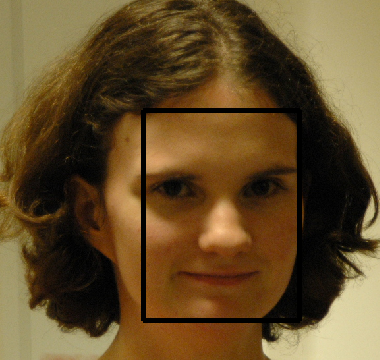
\includegraphics[height=1in]{figures_cvpr/promo/case1/detector.png}&
\hspace{3mm}
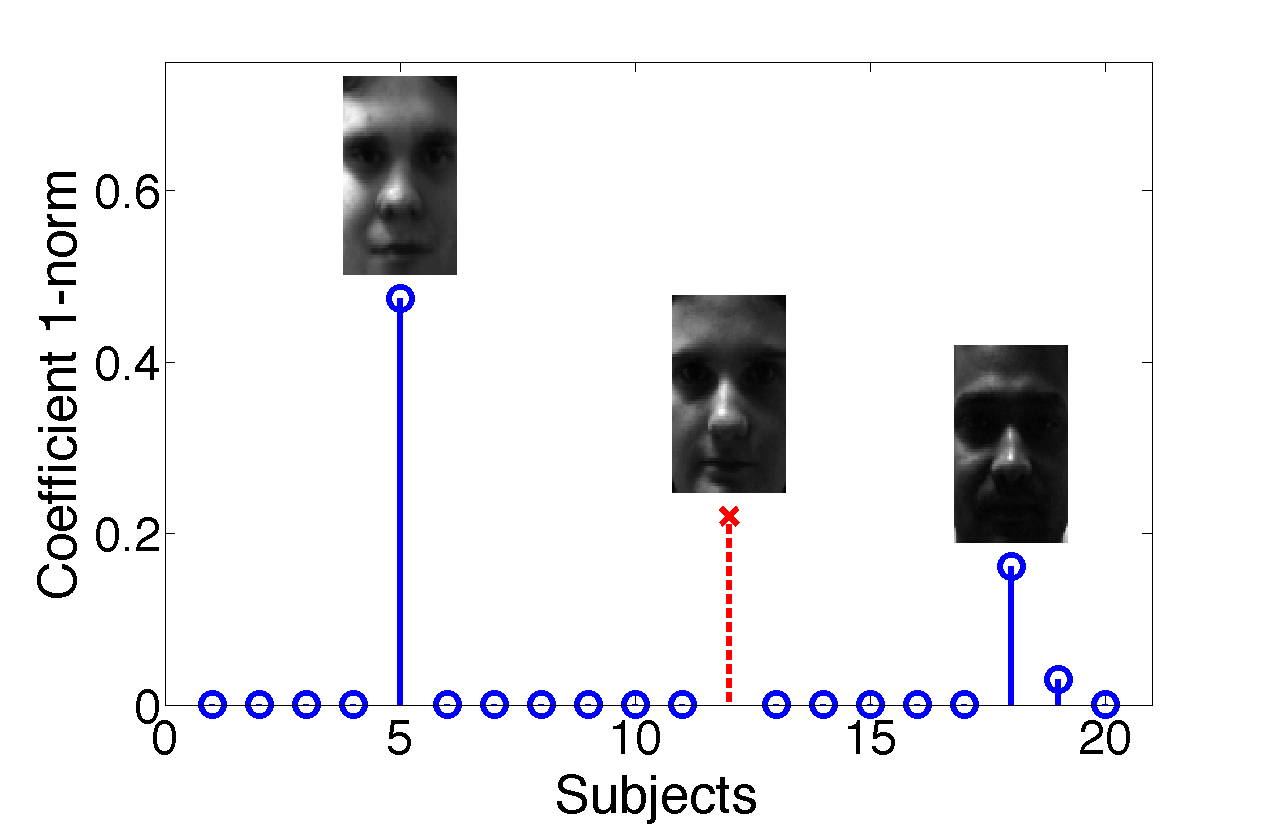
\includegraphics[height=1in]{figures_cvpr/promo/case1/sci_with_axis_face_case1.png}
\\ 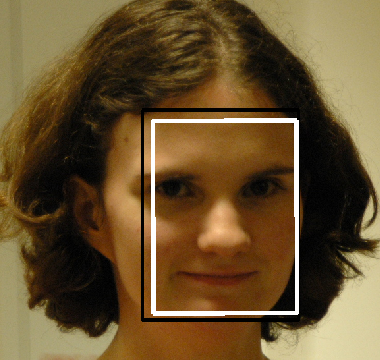
\includegraphics[height=1in]{figures_cvpr/promo/alignment_and_detector.png}&
\hspace{3mm}
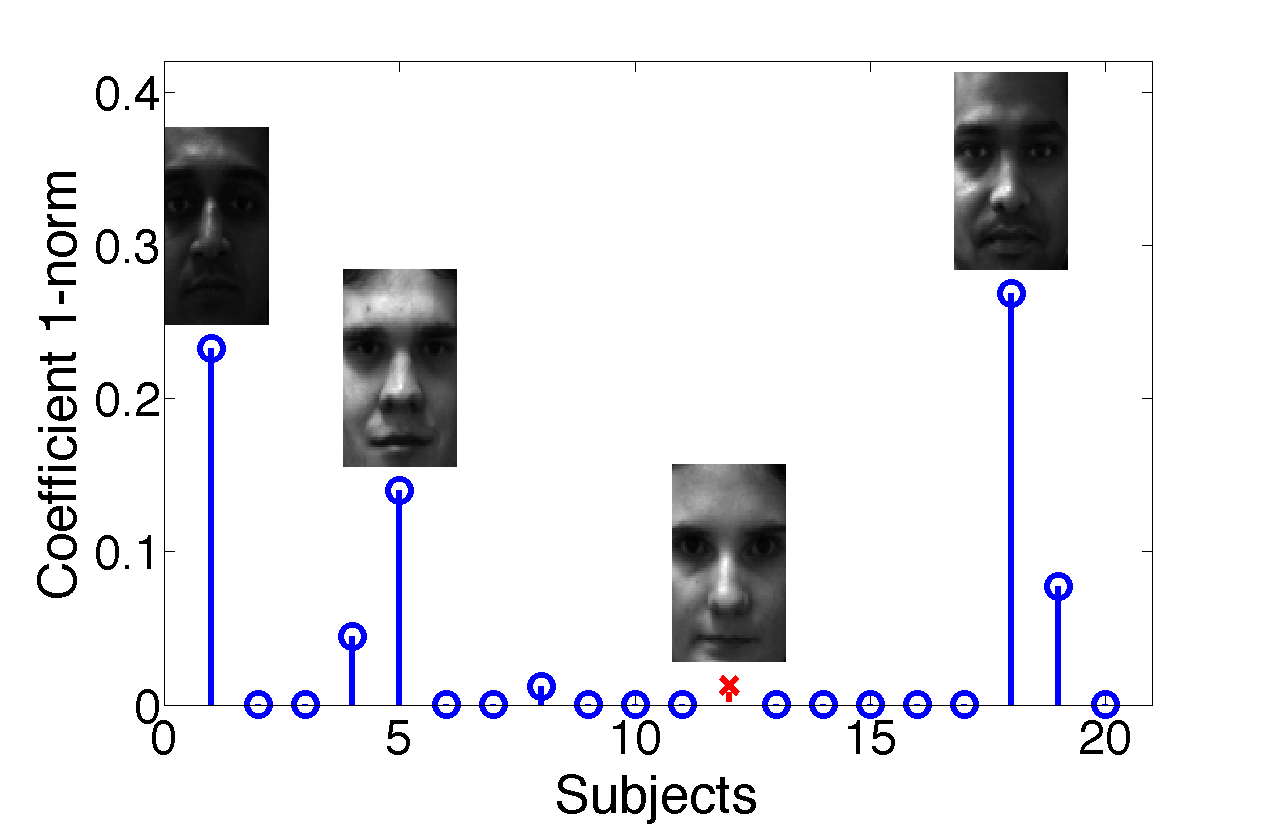
\includegraphics[height=1in]{figures_cvpr/promo/case2/sci_with_axis_face_case2.png}
\\ 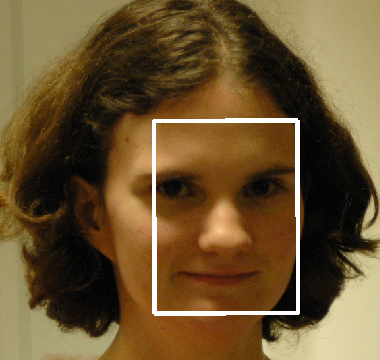
\includegraphics[height=1in]{figures_cvpr/promo/case3/alignment.png} &
\hspace{3mm}
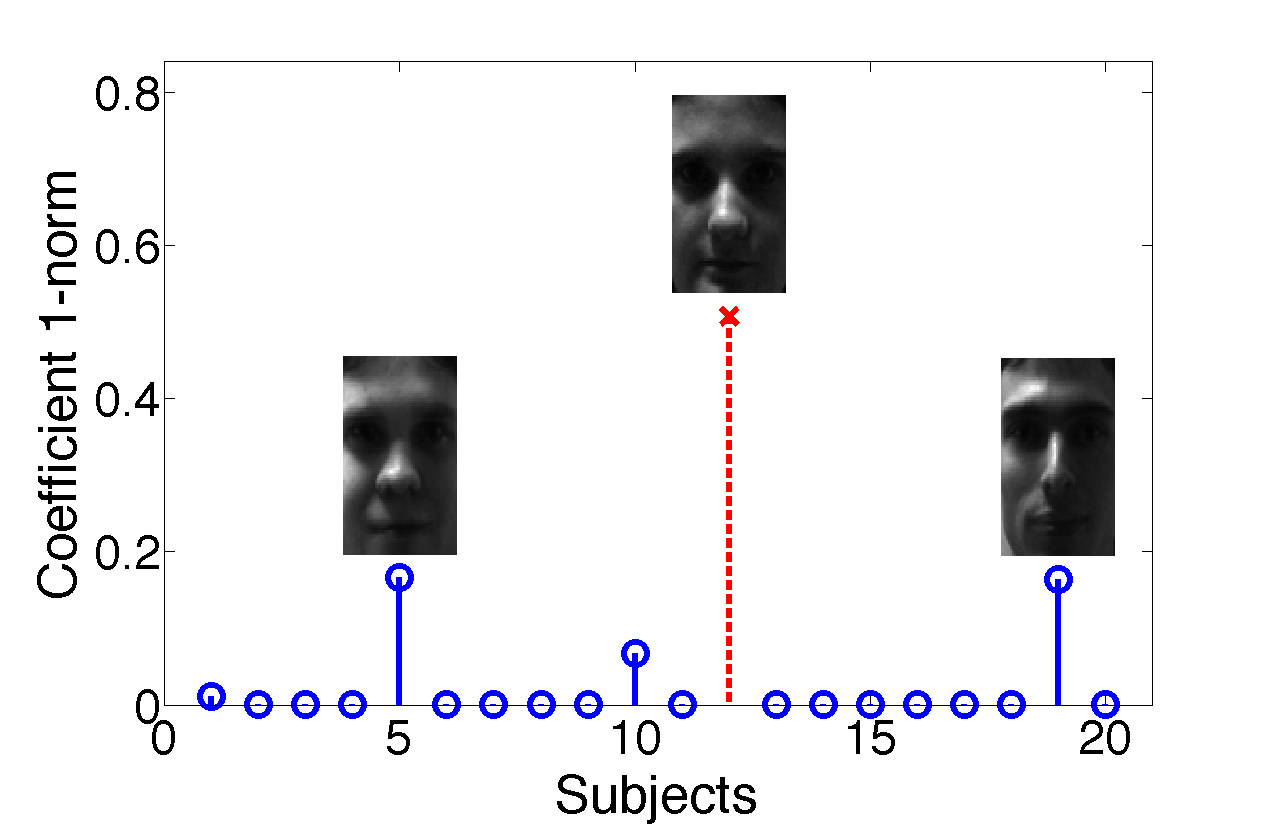
\includegraphics[height=1in]{figures_cvpr/promo/case3/sci_with_axis_face_case3.png}
\end{tabular} \caption{{\bf Effects of registration and illumination on
Recognition}. In this example we identify the girl among 20 subjects, by
computing the sparse representation of her input face with respect to the
entire training set. The absolute sum of the coefficients associated with each
subject is plotted on the right. We also show the faces reconstructed with each
subject's training images weighted by the associated sparse coefficients. The
red line (cross) corresponds to her true identity, subject 12. {\bf Top:} The
input face is from Viola and Jones' face detector (the black box) and all 38
illuminations specified in Section \ref{sec:illumination} are used in the
training.  {\bf Middle:} The input face is well-aligned (the white box) with
the training by our algorithm specified in Section \ref{sec:registration} but
only 24 frontal illuminations are used in the training for recognition (see
Section \ref{sec:illumination}). {\bf Bottom:} The input face is well aligned and
a sufficient set (all 38) of
illuminations are used in the training. Both are necessary for correct recognition
using SRC.}\label{fig:promo}
\vspace{-6.9mm}
\end{figure}

Unfortunately, while the work \cite{Wright2009-PAMI} achieves impressive results, it does not deal with misalignment
between the test and training images, and it requires a rich set of illuminations
in the gallery images for good performance.
We illustrate the compounded effect of both alignment and illumination
with an example in Figure \ref{fig:promo}.
The task is to identify the girl among 20 subjects. If the test
face image, say obtained from an off-the-shelf face detector,
has even a small amount of registration error against the
training images (caused by mild pose, scale, or misalignment),
the sparse representation obtained using the method of \cite{Wright2009-PAMI} is no longer informative,
even if sufficient illuminations are present in the training, as shown in Figure
\ref{fig:promo}(top). Additionally, in order to span
the illuminations of a typical indoor (or outdoor) environment,
illuminations from behind the subject are needed in the
training set. Otherwise, even for perfectly aligned test images,
the sparse representation obtained using \cite{Wright2009-PAMI} will not necessarily be sparse or
informative, as shown by the example in Figure
\ref{fig:promo}(middle). Clearly, both good alignment, as well
as sufficient training images are needed to ensure success of the sparsity-based
recognition method proposed by \cite{Wright2009-PAMI}.
In this paper, we examine how to handle alignment and illumination simultaneously
in the sparse representation framework, bringing the method proposed in \cite{Wright2009-PAMI}
closer to practical use.

\vspace{-0mm}
\subsection{Related Work}
We briefly review existing techniques for recognition, image
registration, and handling of illumination variation.  Our
system is based purely on 2D techniques.  This fact immediately
distinguishes our approach from systems that either require a
3D data as an input, or attempt to estimate a 3D model from 2D
input \cite{amberg2007reconstructing,Blanz2003-PAMI}.  While
these techniques can achieve better robustness to pose
variation given a sufficiently accurate 3D model, for access
control applications where only moderate pose variation is
present, the proposed method will be more than sufficient.
Note that 2D images of faces under varying illuminations
already contain 3D shape-related information,\footnote{In
principle, one can recover the 3D shape of the face from
multiple illuminations using photometric stereo.} and this
information can be leveraged by 2D algorithms for alignment and
recognition even if shape is not reconstructed explicitly.

% Alignment
In holistic recognition algorithms, correspondence between points in the test
image and in the training must be achieved.  A long line of research exists on
using Active Appearance Models \cite{Cootes2001-PAMI}, and the closely related
Active Shape Models \cite{cootes1992active} to register images against a
relatively high-dimensional model of plausible face appearances, often
leveraging face-specific contours.  While these model-based techniques have
advantages in dealing with variations in expression and pose, they may add
unnecessary complexity to applications where subjects normally present a neutral face
or only have moderate expression. We prefer to focus on deformations with far fewer
degrees of freedom, i.e. similarity transformations, and to use the training images themselves
as the appearance model. Iterative registration in this spirit dates at least back to the
Lucas-Kanade algorithm \cite{lucas1981iterative}.

Whereas much of the early work on image registration is aimed at the
problem of registering nearly identical images, say by minimizing a sum of
squared distances or maximizing normalized correlation, here we must confront several physical factors
simultaneously: misalignment, illumination variations, and corrupted pixels.
As we discuss further below, illumination variation can be dealt by
expressing the test image as a linear combination of an appropriate set of
training images. Similar representations have been exploited in
illumination-robust tracking (e.g., \cite{Belhumeur1999-PAA,Murase1995-IJCV}).
For robustness to gross errors, the $\ell^1$-norm of the residual is a more
appropriate objective function than the classical $\ell^2$-norm. Its use here
is loosely motivated by theoretical results due to Cand\`{e}s and Tao
\cite{CandesE2005-IT} (see also \cite{Wright2008-IT}). These two observations
lead us to pose the registration problem as the search for a set of
transformations and illumination coefficients that minimize the $\ell^1$-norm
of the representation error. We solve this problem using a generalized
Gauss-Newton method which solves a sequence of affine-constrained $\ell^1$-norm
minimization problems \cite{Osborne1990-JAMSSB,Jittorntrum1980-NM}. Each of
these problems can also be solved efficiently using recently developed
first-order techniques for $\ell^1$-minimization, which are reviewed in
\cite{YangA2010-pp}.

% Illumination
Researchers have tried various techniques to deal with illumination variation.
In almost all recognition algorithms where only a single gallery image is
available per individual, illumination effects are regarded as a nuisance that
must be removed before the algorithm can continue.  This is typically done by
making statistical assumptions about how illumination affects the image, and
using those assumptions to extract a new representation that is claimed to be
illumination invariant.  Recent examples include \cite{chen2006total} and
\cite{zhou2007appearance}.  However, despite these efforts, truly
illumination-invariant features are difficult to obtain from a single input
image.  We argue that if one has the luxury of designing the acquisition system
and the application demands a high recognition rate,
it is then unwise to limit the gallery to a
single image per person.  We therefore take the strategy of sampling many
gallery images of each individual under varying illuminations.  These images
are used as the basis for either a convex cone model
\cite{Georghiades2001-PAMI,belhumeur1998set}, or a subspace model
\cite{Basri2003-PAMI}.  Images are captured using a simple-to-construct
projector based light stage.  While similar systems have been used for
other applications, to our knowledge, we
are the first to use projectors to indirectly illuminate a subject's face for
the purpose of face recognition.
\subsection{Contributions} In this paper, we show how
registration and illumination
can be simultaneously addressed within a robust sparse representation
framework. We show that face registration, a challenging
nonlinear problem, can be solved by a series of linear programs
that iteratively minimize the sparsity of the registration
error. This leads to an efficient and effective alignment
algorithm for face images that works for a large range of
variation in translation, rotation, and scale, even when
the face is only partially visible due to eyeglasses, closed
eyes and open mouth, sensor saturation, etc.  We also propose a
sufficient set of training illuminations
that is capable of linearly representing typical indoor and outdoor
lighting, along with a practical hardware system for capturing
them.

% The two main contributions of this paper are thus to propose a simple and practical face recognition algorithm that achieves a high degree of robustness and stability to all these variations given sufficient training images, and to demonstrate a practical system for gathering sufficient training images.  While most of the techniques we use have been studied in isolation, we believe we are the first to combine them into a complete recognition pipeline that can achieve good results on realistic data.

% We use tools from sparse representation
% to align a test face image with a set of frontal training
% images in the presence of registration error, illumination variation, and partial occlusion. The region
% of attraction of the alignment algorithm is thoroughly characterized on public face datasets such as Multi-PIE.
% We further demonstrate how to capture a set of training images with enough illumination variation that they span test images taken under un-controlled %illumination.
% We have implemented a complete face recognition system, including a projector-based training acquisition system, in order to evaluate how our algorithms %work under practical testing conditions. We show
% that our system can efficiently and effectively recognize faces under
% a variety of realistic conditions, using only
% frontal images under the proposed illuminations as training.


%This paper is enhanced version of a similarly titled conference paper \cite{Wagner2009-CVPR}.  We provide experiment results on a larger internal data set, as well as more extensive experiments on public data sets.  Furthermore, we test several variations on the main pipeline that also achieve good recognition performance.  We also present an alternative formulation of the iterative alignment based on derivatives of the training images rather than the testing images.  We present results with a new internal implementation of L1 minimization using an Augmented Lagrange Method that is significantly faster than our previous interior-point based solver.


We then demonstrate the effectiveness of the proposed new
methods with a complete face recognition system that is {\em
simple, stable, and scalable}. The proposed system performs
robust automatic recognition of subjects from loosely
controlled probe images taken both indoors and outdoors,
using a gallery of
frontal views of the subjects' faces under the proposed
illuminations. An off-the-shelf face
detector\footnote{We use the OpenCV
implementation of the Viola and Jones' face detector
\cite{Viola2004-IJCV}.} is used to detect faces in the test images.

We conduct extensive experiments on the proposed system with
both public databases and a face database that is collected by
our own acquisition system. Our experimental results on
large-scale public face databases show that our algorithm
indeed achieves very good performance on these databases,
exceeding or competing with the state-of-the-art algorithms.
Additionally, our experimental results on our own database
clearly demonstrate that our system not only works well with
images taken under controlled laboratory conditions, but is
capable of handling practical indoor and outdoor illuminations as well.

\noindent{\em Organization of this paper:} In Section \ref{sec:registration},
we derive our robust registration and recognition algorithm within the sparse
representation framework. We elaborate on algorithmic implementation issues,
conduct region of attraction experiments with respect to both 2D in-plane
deformation and 3D pose variation, and discuss its relationship to existing
work. Section \ref{sec:illumination} is dedicated to our training acquisition
system. Using this system, we investigate empirically how many training
illuminations are required to handle practical illumination variations, and
suggest a sufficient set of 38 training illuminations. Extensive experiments on
a large-scale public database and on our own database are conducted in Section
\ref{sec:multipie} and Section \ref{sec:own-data}, respectively, to verify the
proposed system. Section \ref{sec:conclusion} concludes our work with
discussion of promising future directions.

\section{Robust Alignment}\label{sec:registration}
As demonstrated in Figure \ref{fig:promo}(top), the main
limitation of the {\em sparse representation and
classification} (SRC) algorithm of \cite{Wright2009-PAMI} is
the assumption of pixel-accurate alignment between the test
image and the training set. This leads to brittleness under
pose and misalignment, making it inappropriate for deployment
outside a laboratory setting. In this section, we show how this
weakness can be rectified while still preserving the conceptual
simplicity and good recognition performance of SRC.

SRC assumes access to a database of multiple registered
training images per subject, taken under varying illuminations.
The images of subject $i$, stacked as vectors, form a matrix
$A_i \in \Re^{m \times n_i}$. Taken together, all of the images
form a large matrix $A = [ A_1 \mid A_2 \mid \dots \mid A_K ]
\in \Re^{m \times n}$. As argued in \cite{Wright2009-PAMI}, a
well-aligned test image $\y_0$ can be represented as a sparse
linear combination $A \x_0$ of all of the images in the
database,\footnote{We assume the training illuminations are sufficient. We will address how to ensure illumination
sufficiency in the next section.} plus a sparse error $\e_0$
due to corrupted pixels. The sparse representation can be recovered by
minimizing the $\ell^1$-norm\footnote{The $\ell^1$-norm of a
vector, denoted by $\|\cdot\|_1$, is the sum of absolute values of its entries.} of
$\x$ and $\e$:
\begin{equation}
\min_{\x,\e} \, \| \x \|_1 + \| \e\|_1 \quad \subj \quad \y_0 = A \x + \e.
\label{eqn:robust-l1}
\end{equation}
Now suppose that $\y_0$ is subject to some pose or
misalignment, so that instead of observing $\y_0$, we observe
the warped image $\y = \y_0 \circ \tau^{-1}$, for some
transformation $\tau \in T$ where $T$ is a finite-dimensional
group of transformations acting on the image domain.  The
transformed image $\y$ no longer has a sparse representation of
the form $\y = A \x_0 + \e_0$, and naively applying the
algorithm of \cite{Wright2009-PAMI} is no longer appropriate,
as seen in Figure \ref{fig:promo}(top).

\subsection{Batch and Individual Alignment} If the
true deformation $\tau^{-1}$ can be found, then we can apply
its inverse $\tau$ to the test image and it again becomes
possible to find a sparse representation of the resulting
image, as $\y \circ \tau = A \x_0 + \e_0$.\footnote{In the terminology of \cite{baker2004lucas}, this formulation is ``Forward Additive''.}
  This sparsity
provides a strong cue for finding the correct deformation
$\tau$: conceptually, one would like to seek a transformation
$\tau$ that allows the sparsest representation, via
\begin{equation} \label{eqn:L1-L1-conceptual}
\hat{\tau} = \arg\hspace{-2.5mm}\min_{\x,\e,\tau \in T} \| \x \|_1 + \| \e \|_1 \quad \subj \quad \y \circ \tau = A \x + \e.
\end{equation}
For fixed $\tau$, this problem is jointly convex in $\x$ and
$\e$. However, as a simultaneous optimization over the
coefficients $\x$, error representation $\e$, and
transformation $\tau$, it is a difficult, nonconvex
optimization problem. One source of difficulty is the presence
of multiple faces in the matrix $A$:
\eqref{eqn:L1-L1-conceptual} has many local minima that
correspond to aligning $\y$ to different subjects. In this
sense, the misaligned recognition problem differs from the
well-aligned version studied in \cite{Wright2009-PAMI}. For the
well-aligned case, it is possible to directly solve for a
global representation, with no concern for local minima. With
possible misalignment, it is more appropriate to seek the best
alignment of the test face with each subject $i$:
\begin{equation} \label{eqn:per-subject-L1}
\hat \tau_i = \arg\hspace{-2.5mm}\min_{\x,\e,\tau_i \in T} \| \e \|_1 \quad \subj \quad \y \circ \tau_i = A_i \x + \e.
\end{equation}
We no longer penalize $\| \x \|_1$, since $A_i$ consists of
only images of subject $i$ and so $\x$ is no longer expected to
be sparse.

\subsection{Alignment via Sequential $\ell^1$-Minimization} While the problem \eqref{eqn:per-subject-L1} is still nonconvex, for cases of practical interest in face recognition, a good initial guess for the transformation is available, e.g., from the output of a face detector. We can refine this initialization to an estimate of the true transformation by repeatedly linearizing about  the current estimate of $\tau$, and seeking representations of the form:
\begin{equation}
\y\circ \tau + J \Delta \tau = A_i \x + \e.
\end{equation}
Here, $J = \frac{\partial}{\partial \tau} \y \circ \tau$ is the
Jacobian of $\y \circ \tau$ with respect to the transformation
parameters $\tau$, and $\Delta \tau$ is the step in $\tau$. The
above equation is underdetermined if we allow the registration
error $\e$ to be arbitrary. At the correct alignment we
expect the test image to differ from $A_i \x$ only
for the minority of the pixels corrupted by occlusions. Thus,
we seek a deformation step $\Delta \tau$ that best sparsifies the registration error $\e$, in terms of its $\ell^1$-norm:
\begin{equation}
\Delta\hat{\tau}_1 = \arg\hspace{-3.5mm}\min_{\x,\e,\Delta\tau \in T} \| \e \|_1 \quad \subj \quad \y\circ\tau + J \Delta \tau = A_i \x + \e.
\label{eqn:L1-align}
\end{equation}
This is different from the popular choice that
minimizes the $\ell^2$-norm of the registration error:
\begin{equation}
\Delta\hat{\tau}_2 = \arg\hspace{-3.5mm}\min_{\x,\e,\Delta\tau \in T} \| \e \|_2 \quad \subj \quad \y\circ\tau + J \Delta \tau = A_i \x + \e,
\label{eqn:L2-align}
\end{equation}
which is also equivalent to finding the deformation step
$\Delta  \tau$ by solving the least-square problem:
$\min_{\x,\Delta \tau} \|\y \circ \tau + J\Delta \tau - A_i \x
\|_2$. Empirically, we find that if there is only small noise
between $\y_0$ and $A_i\x$, both \eqref{eqn:L1-align} and
$\eqref{eqn:L2-align}$ have similar performance.  However, if
there are occlusions in $\y_0$, sequential
$\ell^1$-minimization \eqref{eqn:L1-align} is significantly
better than sequential $\ell^2$-minimization
\eqref{eqn:L2-align}. Figure \ref{fig:L1-L2-align} shows an
example.

The scheme \eqref{eqn:L1-align} can be viewed as a generalized Gauss-Newton method for minimizing the composition of a nonsmooth objective function (the $\ell^1$-norm) with a differentiable mapping from transformation parameters to transformed images. Such algorithms date at least back to the 1970's  \cite{Cromme1978-NM,Jittorntrum1980-NM}, and continue to attract attention today \cite{Lewis2008-TR}. While space precludes a detailed discussion of their properties, we should mention that the scheme \eqref{eqn:L1-align} is known to converge quadratically in the neighborhood of any local optimum of the $\ell^1$-norm. In practice, this means that $\approx$ 10 to 15 iterations suffice to reach the desired solution. We refer the interested reader to \cite{Jittorntrum1980-NM,Osborne1990-JAMSSB} and the references therein.

\begin{figure}
\centering
{\small
\begin{tabular}{cccc}
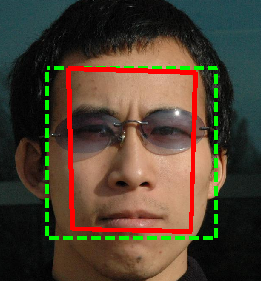
\includegraphics[height=.8in]{figures_cvpr/L1_cropped} &

\includegraphics[height=.8in]{figures_cvpr/y_warp_L1} &

\includegraphics[height=.8in]{figures_cvpr/y_hat_L1} &

\includegraphics[height=.8in]{figures_cvpr/e_L1} \\
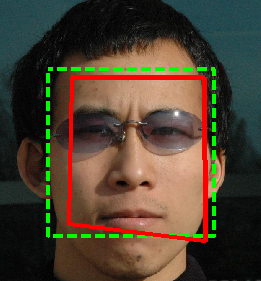
\includegraphics[height=.8in]{figures_cvpr/L2_cropped} &

\includegraphics[height=.8in]{figures_cvpr/y_warp_L2} &

\includegraphics[height=.8in]{figures_cvpr/y_hat_L2} &

\includegraphics[height=.8in]{figures_cvpr/e_L2} \\
(a) & (b) & (c) & (d)
\end{tabular}
\vspace{0mm}}
\caption{{\bf Comparing alignment of a subject wearing sunglasses by
$\ell^1$ and $\ell^2$ minimization.}
{\bf Top:} alignment result of minimizing $\|\e\|_1$; {\bf Bottom:}
result of minimizing $\|\e\|_2$. (a) {\em Green (dotted):} Initial face boundary
given by the face detector, {\em Red (solid):} Alignment result shown on the same
face; (b) warped testing image using the estimated transformation $\y_0$;
(c) reconstructed face $A_i\x$ using the training; (d) image of error $\e$. }\label{fig:L1-L2-align}
\vspace{-8.0mm}
\end{figure}

In addition to normalizing the training images (which is done
once), it is important to normalize the warped testing image
$\y \circ \tau$ as the algorithm runs.  Without normalization,
the algorithm may fall into a degenerate global minimum
corresponding to zooming in on a dark region of the test
image.  Normalization is done by replacing the linearization of
$\y \circ \tau$ with a linearization of the normalized version
$\tilde \y(\tau) = \frac{\y \circ \tau}{\|\y \circ \tau\|_2}$.
The proposed alignment algorithm can be easily extended to work
in a {\em multiscale} fashion, with benefits both in
convergence behavior and computational cost.  The alignment
algorithm is simply run to completion on progressively less
downsampled versions of the training and testing images, using
the result of one level to initialize the next.

\subsection{Robust Recognition by Sparse Representation} Once
the best transformation $\tau_i$ has been computed for each
subject $i$, the training sets $A_i$ can be aligned to $\y$,
and a global sparse representation problem of the form
\eqref{eqn:robust-l1} can be solved to obtain a discriminative
representation in terms of the entire training set. Moreover,
the per-subject alignment residuals $\| \e \|_1$ can be used to
prune unpromising candidates from the global optimization,
leaving a much smaller and more efficiently solvable problem.
The complete optimization procedure is summarized as Algorithm
\ref{alg:deformable-src}. The parameter $S$ in our algorithm is the number of subjects
considered together to provide a sparse representation for the
test image. If $S = 1$, the algorithm reduces to classification
by registration error; but considering the test image might be
an invalid subject, we typically choose $S = 10$. Since valid
images have a sparse representation in terms of this larger
set, we can reject invalid test images using the {\em sparsity
concentration index} proposed in \cite{Wright2009-PAMI}.
The function $\delta_i(\x)$ in Algorithm \ref{alg:deformable-src}
selects coefficients from the vector $\x$ corresponding to subject $i$.

Another important free parameter in Algorithm
\ref{alg:deformable-src} is the class of deformations $T$. In
our experiments, we typically use 2D similarity
transformations, $T = \mathbb{SE}(2)\times \Re_+$\footnote{Here, SE stands for Special
Euclidean, i.e., 2D rigid transformations.  The $\Re_+$ accounts for the scale.}, for removing alignment error incurred by face
detector, or 2D projective transformations, $T =
\mathbb{GL}(3)\footnote{Here, GL stands for General Linear.
This class of transformations is able to represent distortion
in a perspective image of a planar object.}$, for handling some
pose variation.

In Algorithm \ref{alg:deformable-src}, we also implement a simple heuristic which improves the
performance of our system, based on the observation that the face detector output may be poorly centered on
the face, and may contain a significant amount of the background.  Therefore, before the recognition stage,
instead of aligning the training sets to the
original $\y$ directly obtained from the face detector, we
compute an average transformation $\bar{\tau}$ from $\tau_{k_1},
\tau_{k_2}, \ldots, \tau_{k_S}$ of the top $S$ classes, which
is believed to be better centered, and update $\y$ according to
$\bar{\tau}$. For the 2D similarity transformations, which are
used in our system when initialized by the face detector, a
transformation $\tau$ can be parameterized as $\tau = (\tau^1,
\tau^2, \tau^3, \tau^4)$, where $\tau^1$ and $\tau^2$ represent
the translations in $x$- and $y$-axis, $\tau^3$ represents the
rotation angle and $\tau^4$ represents the scale. Then the
average transformation is simply obtained by taking the
component-wise mean:
\begin{displaymath}
\bar{\tau}^i = (\tau_{k_1}^i + \tau_{k_2}^i + \cdots +
\tau_{k_S}^i) / S, i = 1,2,3,4.
\end{displaymath}
Finally, the training sets are aligned to the new $\y$.

\begin{algorithm}[thb]
\caption{\bf (Deformable Sparse Recovery and Classification for
Face Recognition)} \label{alg:deformable-src}
\begin{algorithmic}[1]
\begin{small}
\STATE {\bf Input:} Training images $\{A_i \in \Re^{m\times n_i}\}_{i=1}^K$ for $K$ subjects,  a test image
$\y\in\Re^m$ and a deformation group $T$.
\STATE
{\bf for} each subject $i$,
\STATE \hspace{3mm} $\tau^{(0)}
\leftarrow I$.
\STATE \hspace{3mm} {\bf while} not converged $(j=1,2,\ldots)$ {\bf do}
\STATE \hspace{6mm}
$\tilde \y(\tau) \leftarrow \frac{\y \circ \tau}{\|\y \circ
\tau\|_2}$; \;\;\; $J \leftarrow  \frac{\partial}{\partial
\tau} \tilde\y(\tau)  \bigr|_{\tau^{(j)}} $;
%\STATE \hspace{6mm} $(\hat \x, \hat \e, \Delta \tau) \leftarrow \left\{\begin{array}{l} \arg \min_{\x,\e,\Delta \tau} \| \e \|_1 \\  \subj \; \y + J \Delta \tau = A_k \x + \e \end{array}\right.$
\STATE \hspace{6mm} $ \Delta \tau =  \arg\min \; \| \e \|_1  \;
\subj \; \tilde \y + J \Delta \tau = A_i \x + \e.$
\STATE
\hspace{6mm} $\tau^{(j+1)} \leftarrow \tau^{(j)} + \Delta
\tau$;
\STATE \hspace{3mm} {\bf end while} \STATE {\bf end} \STATE Keep
the top $S$ candidates $k_1, \ldots, k_S$ with the smallest
residuals $\|\e\|_1$. \STATE Compute an average transformation
$\bar{\tau}$ from $\tau_{k_1}, \tau_{k_2}, \ldots, \tau_{k_S}$.
\STATE Update $\y \leftarrow \y \circ \bar{\tau}$ and $\tau_i
\leftarrow \tau_i \cdot \bar{\tau}^{-1}$ for $i = k_1, \dots,
k_S$. \STATE Set $A \leftarrow \big[ A_{k_1} \circ
\tau_{k_1}^{-1} \mid A_{k_2} \circ \tau_{k_2}^{-1} \mid \dots
\mid A_{k_S} \circ \tau_{k_S}^{-1} \big]$. \STATE Solve the
$\ell^1$-minimization problem: \hspace{2mm}
$\hat{\x} = \arg \min_{\x, \e} \| \x \|_1 + \|\e\|_1 \;\; \subj \;\; \y = A \x + \e.$
\STATE Compute residuals $r_i(\y) = \| {\y} - {A}_i \, \delta_i(\hat{\x}) \|_2$ for $i = k_1, \dots, k_S$.
\STATE {\bf Output:} $\mbox{identity}(\y) = \arg\min_i r_i(\y)$.
\end{small}
\end{algorithmic}
\end{algorithm}
%\vspace{-4mm}

The transformation $\tau$ defines a mapping between the
coordinates of pixels in the large original image and a smaller
(un)warped image. The pixels of the small image are stacked into a vector. To prevent aliasing
artifacts in the downsampled image, one should apply a
smoothing filter to the original image. For a simple implementation, a rectangular window with
regular sampling can used, but in general, the small image need
not be regularly sampled in pixel coordinates.  For example,
the sample locations could be arbitrarily selected from within a
``face shaped'' area. We will discuss how choosing
different windows can affect the performance of our algorithm
in Section \ref{sec:multipie}.

\subsection{System Implementation}
In this section, we discuss the computational issues related to
the implementation of Algorithm~\ref{alg:deformable-src}. It is
not hard to see that its computational complexity is dominated
by the two steps where the $\ell^1$-norm minimization problems
are solved; namely Step 6 for iterative registration, and Step
14 for global sparse representation.
Fortunately, many fast algorithms for solving these problems have been proposed over the
past ten years. We refer the interested reader to \cite{YangA2010-pp} for a more comprehensive survey of the developments in this area.
That work suggests that \emph{Augmented Lagrange Multiplier}
(ALM) algorithms \cite{Bertsekas1982} strike a good balance
between scalability and accuracy: as first order methods, they
require only lightweight vector operations and matrix-vector
multiplications at each iteration, making them preferable to
more classical solutions such as interior point methods.
However, compared to other first-order methods, they achieve
higher accuracy with a fixed computational budget.

We use Step 14 as an example to illustrate the ALM
method, since solving Step 6 is very similar. Recall that in
Step 14 the problem we are interested in is:
\begin{equation}
\min_{\x, \e} \| \x \|_1 + \|\e\|_1 \quad \subj \quad \y =
A \x + \e.
\end{equation}
Its corresponding augmented Lagrangian function is
\begin{equation}
L_\mu (\x,\e,\blamda) = \|\x\|_1 + \|\e\|_1 + \langle \blamda, \y-A\x - \e \rangle + \frac{\mu}{2} \|\y - A\x - \e\|_2^2,
\end{equation}
where $\blamda$ is the Lagrange multiplier and $\mu > 0$ is a
penalty parameter. The ALM method seeks a saddlepoint of $L_\mu
(\x,\e,\blamda)$ by alternating between optimizing with respect
to the primal variables $\x, \e$ and updating the dual variable
$\blamda$, with the other fixed, as follows:
\begin{equation}
\left \{
\begin{array}{lll}
(\x_{k+1},\e_{k+1})  =  \arg\min_{(\x,\e)} \, L_{\mu} (\x,\e,\blamda_k),\\
\blamda_{k+1}  =  \blamda_k + \mu (\y - A\x_{k+1} - \e_{k+1}). \\
\end{array}
\right .
\label{eq:alm}
\end{equation}
Although updating $\blamda$ is trivial,
minimizing $L_{\mu} (\x,\e,\blamda_k)$ with respect to both
$\x$ and $\e$ could still be costly. To further reduce the
complexity of the problem, we adopt an approach used in
\cite{YangJ2009-pp}, called \emph{alternating direction
method of multipliers} (ADM) \cite{Glowinski1975-TR}, which alternates between minimizing $L_{\mu} (\x,\e,\blamda_k)$
over $\x$ (with $\e$ fixed) and over $\e$ (with $\x$ fixed). After solving these two subproblems, the Lagrange multiplier $\blamda$ is updated, yielding an iteration of the form:
\begin{equation}
\left \{
\begin{array}{lll}
\e_{k+1}  =  \arg\min_{\e} \, L_{\mu} (\x_k,\e,\blamda_k),\\
\x_{k+1}  =  \arg\min_{\x} \, L_{\mu} (\x,\e_{k+1},\blamda_k),\\
\blamda_{k+1}  =  \blamda_k + \mu (\y - A\x_{k+1} - \e_{k+1}). \\
\end{array}
\right .
\label{eq:adm}
\end{equation}
As the objective function is convex and alternation is between two
terms, this procedure is guaranteed to converge to a global optimum (see \cite{YangJ2009-pp} and references therein).

In order to discuss the solution to the above subproblems, we
need to define the following soft-thresholding operator for a
vector $\x$ and a scalar $\alpha \geq 0$:
\begin{equation}
\mathcal{T}(\x,\alpha) = \textup{sign}(\x)\cdot \max \{|\x| - \alpha, 0\},
\end{equation}
where all the operations are performed component-wise. It is
easy to show that the subproblem with respect to $\e$ has a
closed-form solution given by the soft-thresholding operator:
\begin{equation}
\e_{k+1} = \mathcal{T}(\y - A\x_k + \mu^{-1}\blamda_k, \mu^{-1}).
\end{equation}
To solve the subproblem associated with $\x$, we
apply a first-order $\ell^1$-minimization method,
called \emph{fast iterative shrinkage-threshold algorithm}
(FISTA) \cite{BeckA2009}. The main idea of FISTA is to
iteratively minimize a quadratic approximation $Q(\x, \z)$ to
$L_{\mu} (\x,\e_{k+1},\blamda_k)$ around a point $\z$, which is
carefully chosen in order to achieve a good convergence
rate. We summarize the entire ALM
algorithm as Algorithm~\ref{alg:alm}, where $\gamma$ denotes the
largest eigenvalue of the matrix $A^TA$. For the choice of parameter $\mu$, we take the same strategy as
in \cite{YangJ2009-pp} and set $\mu = 2m / \|\y\|_1$.
\begin{algorithm}[t]
\caption{\bf (Augmented Lagrange Multiplier Method for Global
Recognition)}
\begin{algorithmic}[1]
\begin{small}
\STATE {\bf Input:} $\y \in \Re^m$, $A \in \Re^{m \times n}$,
$\x_1 = \mathbf{0}$, $\e_1 = \y$, $\blamda_1 =
\mathbf{0}$.
\WHILE{not converged ($k = 1,2,\ldots$)}
\STATE $\e_{k+1} = \mathcal{T}\left(\y - A\x_k +
\frac{1}{\mu}\blamda_k, \frac{1}{\mu}\right)$;
\STATE $t_1\leftarrow 1$, $\z_1 \leftarrow \x_k$, $\w_1 \leftarrow \x_k$;
\WHILE{not converged ($l = 1,2,\ldots$)}
\STATE $\w_{l+1} \leftarrow \mathcal{T}\left(\z_l +
\frac{1}{\gamma}A^T\left(\y - A\z_l - \e_{k+1} +
\frac{1}{\mu}\blamda_k\right), \frac{1}{\mu\gamma}\right)$;
\STATE $t_{l+1} \leftarrow \frac{1}{2}\left( 1 +
\sqrt{1+4t_l^2}\right)$;
\STATE $\z_{l+1} \leftarrow \w_{l+1} + \frac{t_l - 1}{t_{l+1}}(\w_{l+1} - \w_l)$;
\ENDWHILE
\STATE $\x_{k+1} \leftarrow \w_{l}$,  \; $\blamda_{k+1} \leftarrow \blamda_k + \mu (\y - A\x_{k+1} - \e_{k+1})$;
\ENDWHILE \STATE
{\bf Output:} $\x^* \leftarrow \x_k, \e^* \leftarrow \e_k$.
\end{small}
\end{algorithmic}
\label{alg:alm}
%\vspace{-4mm}
\end{algorithm}

We have selected this algorithm because it strikes the best
balance between speed, accuracy, and scalability for our problem out of
many algorithms that we have tested. We refer the interested reader to
\cite{YangA2010-pp} for a more detailed discussion of competing
approaches.  On a Mac Pro with
Dual-Core 2.66GHz Xeon processors and 4GB memory,
running on our database containing images size $80\times 60$
pixels from 109 subjects under 38 illuminations,
our C implementation of Algorithm~\ref{alg:deformable-src} takes
about 0.60 seconds per subject for alignment and about 2.0
seconds for global recognition. Compared to the highly
customized interior point method used in the conference version
of this paper \cite{Wagner2009-CVPR}, this new algorithm is
only slightly faster for per subject alignment. However, it is
much simpler to implement and it achieves a
\emph{speedup of more than a factor of 10} for global
recognition!

\subsection{Experiments on Region of Attraction} We will now present three
experimental results demonstrating the effectiveness of the individual
alignment procedure outlined in the previous section. They show the sufficiency
of the region of attraction, verify effectiveness of the multiscale extension,
and show stability to small pose variations.  We delay large-scale recognition
experiments to Sections \ref{sec:multipie} and \ref{sec:own-data}, after we
have discussed the issue of illumination in the next section.

\noindent {1) \em 2D Deformation.}  We first verify the
    effectiveness of our alignment algorithm with images
    from the CMU Multi-PIE Database \cite{Gross2008-FGR}.
    We select all the subjects in Session 1, use 7
    illuminations per person from Session 1 for training,
    and test on one new illumination from Session
    2.\footnote{The training are illuminations $\{0, 1, 7,
    13, 14, 16, 18\}$ of \cite{Gross2008-FGR}, and the
    testing is the illumination 10. } We manually select
    eye corners in both training and testing as the ground
    truth for registration. We downsample the images to
    $80\times 60$ pixels\footnote{Unless otherwise stated,
    this will be the default resolution at which we prepare
    all our training and testing datasets.} and the distance between the two outer
    eye corners is normalized to be 50 pixels for each
    person. We introduce artificial deformation to the
    testing image with a combination of translation,
    rotation and scaling. We further use the alignment
    error $\|\e\|_1$ as an indicator of success. Let $r_0$
    be the alignment error obtained by aligning a test
    image to the training images without any artificial
    perturbation. When the test image is artificially
    perturbed and aligned, resulting in an alignment error
    $r$, we consider the alignment successful if $|r - r_0 | \leq
    0.01r_0$. Figure \ref{fig:attraction} shows the
    percentage of successful registrations for all subjects
    for each artificial deformation. The results suggest
    that our algorithm works extremely well with
    translation up to 20\% of the eye distance (or 10
    pixels) in all directions and up to $30^\circ$ in-plane
    rotation. We have also tested our alignment algorithm
    with scale variation and it can handle up to 15\%
    change in scale.

We have gathered the statistics of the Viola and Jones'
 face detector on the Multi-PIE dataset. For 4,600 frontal
 images of 230 subjects under 20 different illuminations,
 using manual registration as the ground truth, the average
 misalignment error of the detected faces is about 6 pixels
 and the average variation in scale is 8\%. This falls
 safely inside the region of attraction for our alignment
 algorithm.
\begin{figure*}
\centering
{\small
\begin{tabular}{ccc}
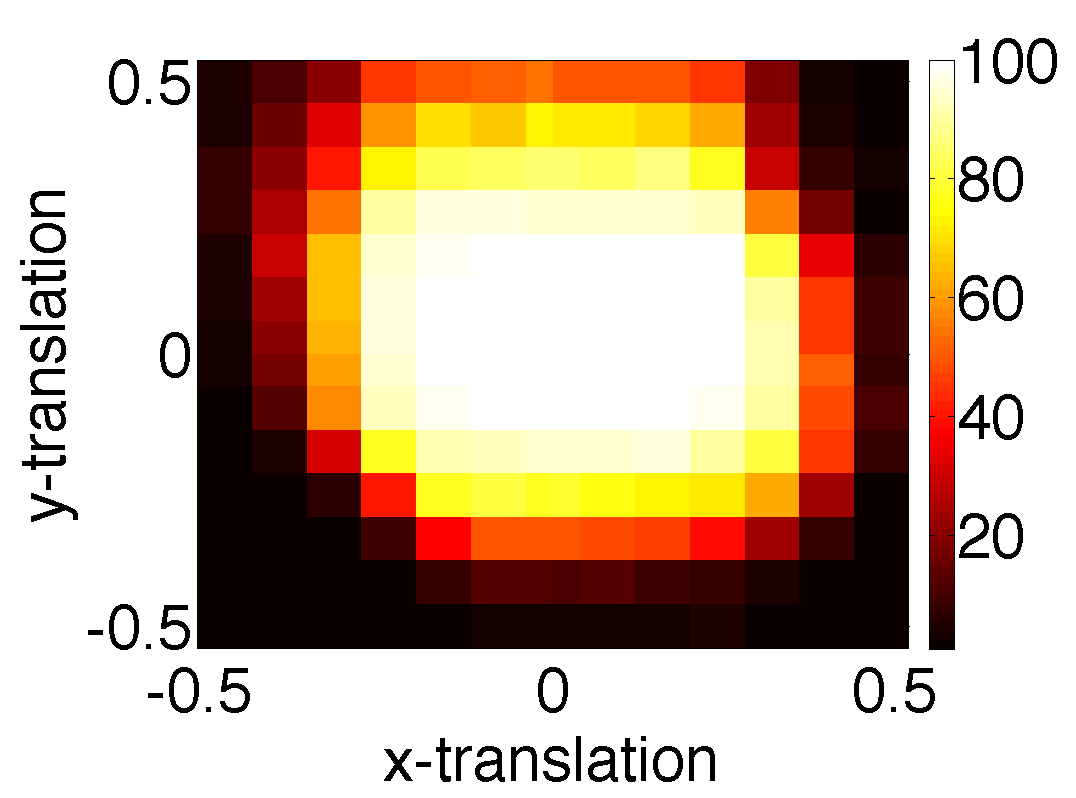
\includegraphics[height=1.2in]{figures_pami/x_y_roa.png} &
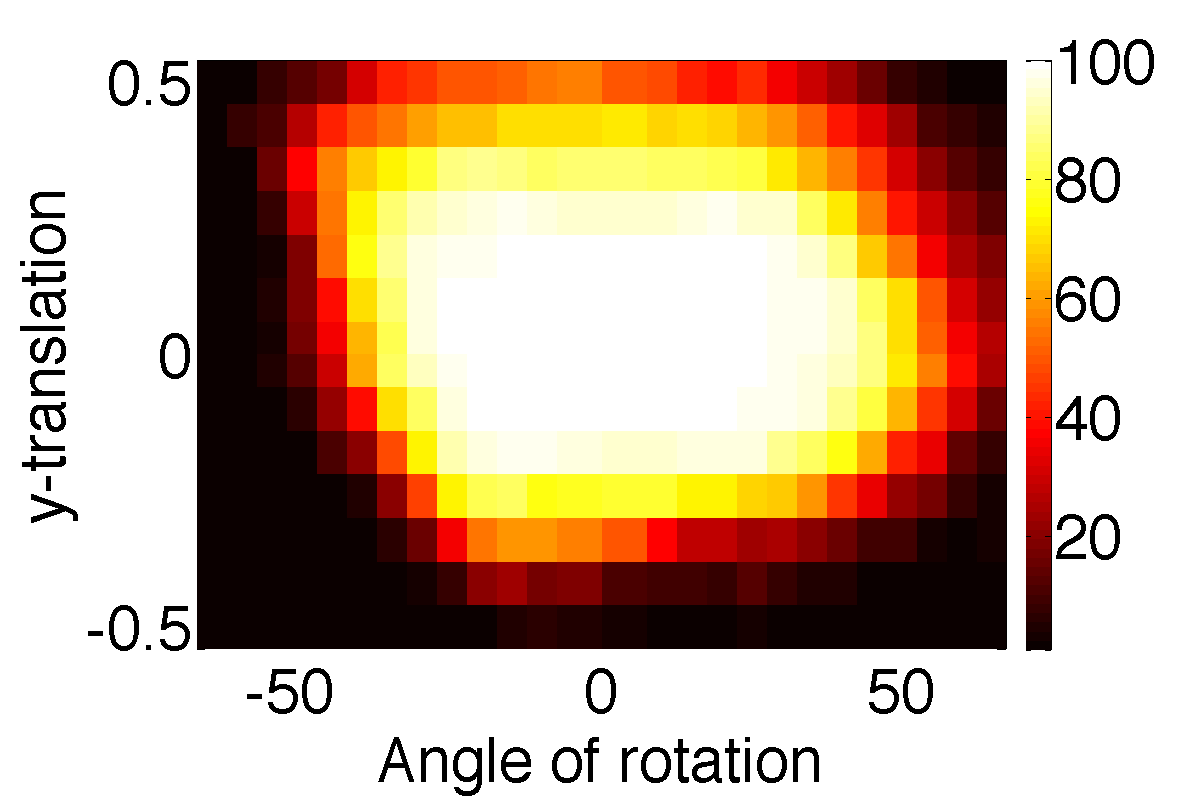
\includegraphics[height=1.2in]{figures_pami/y_theta_roa.png} &
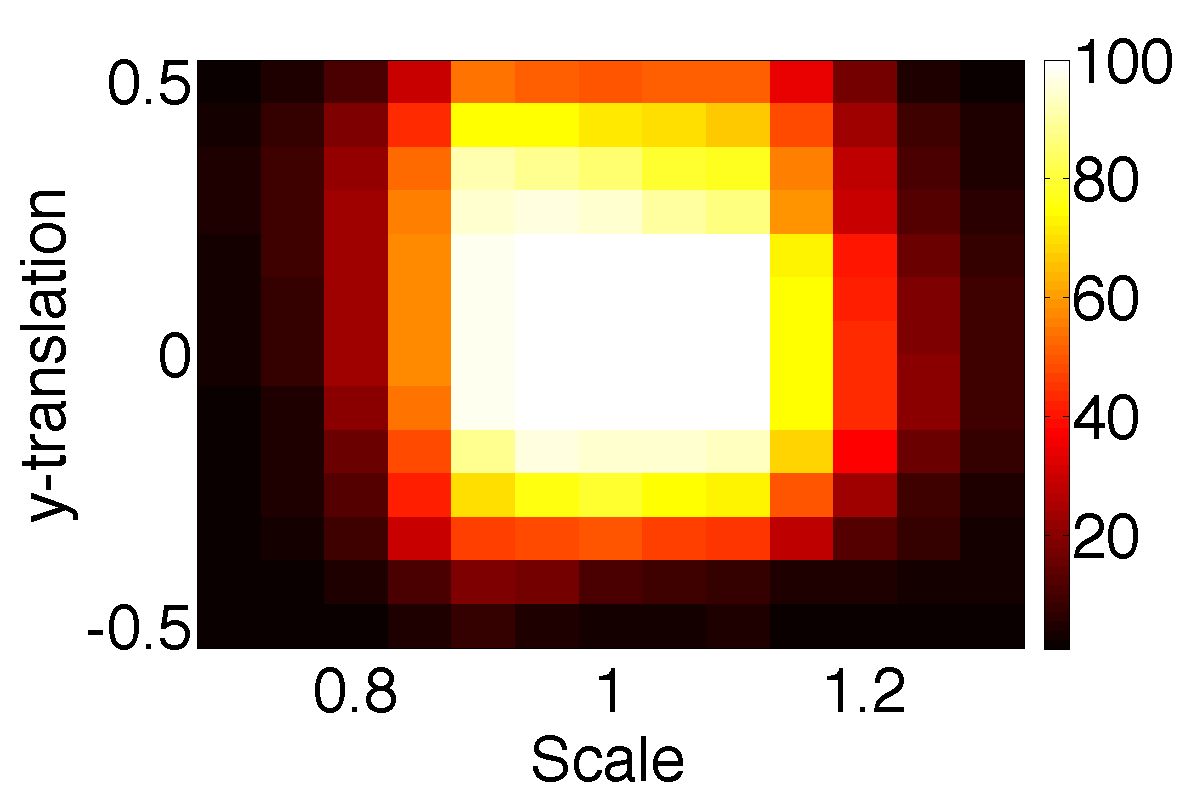
\includegraphics[height=1.2in]{figures_pami/y_s_roa.png}\\
(a)&(b)&(c)
\end{tabular}
\begin{tabular}{cccc}
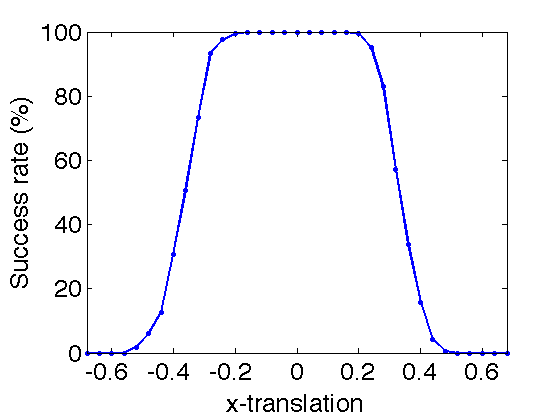
\includegraphics[height=1in]{figures_pami/x_tr.png} &
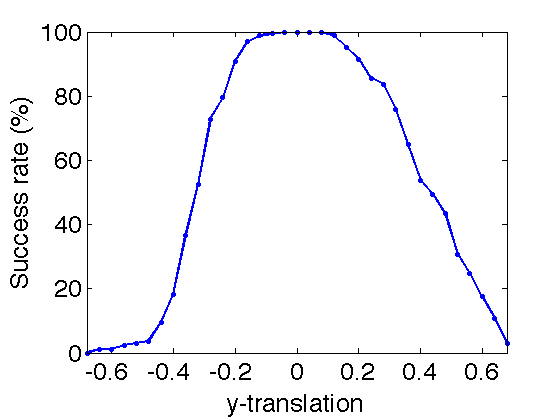
\includegraphics[height=1in]{figures_pami/y_tr.png} &
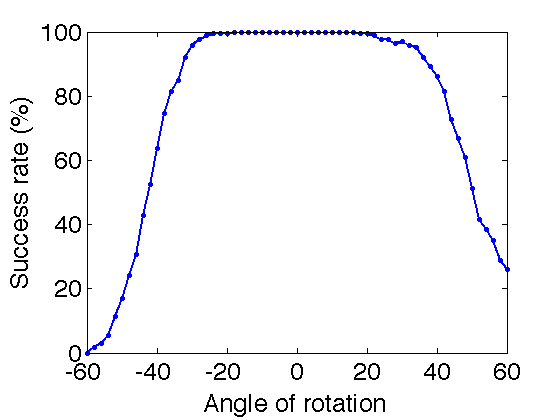
\includegraphics[height=1in]{figures_pami/theta.png} &
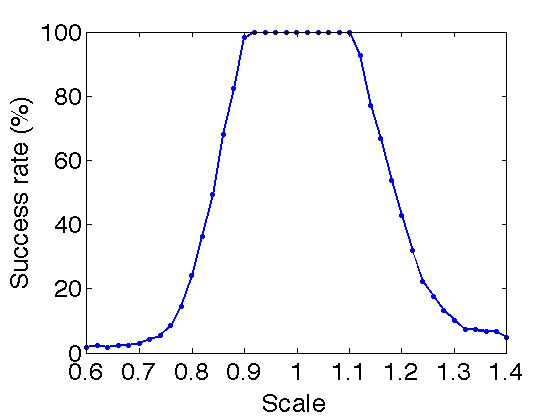
\includegraphics[height=1in]{figures_pami/scale.png}\\
(d)&(e)&(f)& (g)
\end{tabular}
\vspace{0mm}
}
\caption{{\bf Region of attraction.} Fraction of subjects for which the algorithm successfully aligns a synthetically perturbed test image.  The amount of translation is expressed as a fraction of the distance between the outer eye corners, and the amount of in-plane rotation in degrees. {\bf Top row:} (a) Simultaneous translation in $x$ and $y$ directions. (b) Simultaneous translation in $y$ direction and in-plane rotation. (c) Simultaneous translation in $y$ direction and scale variation. {\bf Bottom row:} (d) Translation in $x$ direction only. (e) Translation in $y$ direction only. (f) In-plane rotation only. (g) Scale variation only.}
\label{fig:attraction}
\vspace{0mm}
\end{figure*}

\noindent{2) \em Multiscale Implementation.}
Performing alignment in a multiscale fashion has two benefits: first, it provides a larger region of attraction, and second, it reduces overall computational cost. Here, we further investigate the convergence behavior of the algorithm as a function of the standard deviation $\sigma$ of the Gaussian smoothing filter and the number of scales considered.
We use the same 7 illuminations in
Session 1 as training, and all 20 illuminations in the same
session as testing. We introduce artificial deformation in
both $x$ and $y$ directions up to 16 pixels in the
$80\times 60$ frame, with a step size of 4 pixels, i.e.,
$(\Delta x, \Delta y) \in \{-16,-12,\ldots,12,16\} \times
\{-16,-12,\ldots,12,16\}$. We consider an alignment
successful if the estimated coordinates of the eye-corners
are within 1 pixel from the ground truth in the original
image.  In Figure \ref{fig:multiscale}, we report the
alignment success rate, averaged over the artificially
perturbed initial deformations, as a function of the
standard deviation of the Gaussian kernel $\sigma$, for
three choices of the number of scales. As one can see,
using multiscale indeed improves the performance, and when
3 scales are used, a smaller convolution kernel can achieve
a similar performance compared to a much larger kernel when
only 2 scales are used.
\begin{figure}
\centering
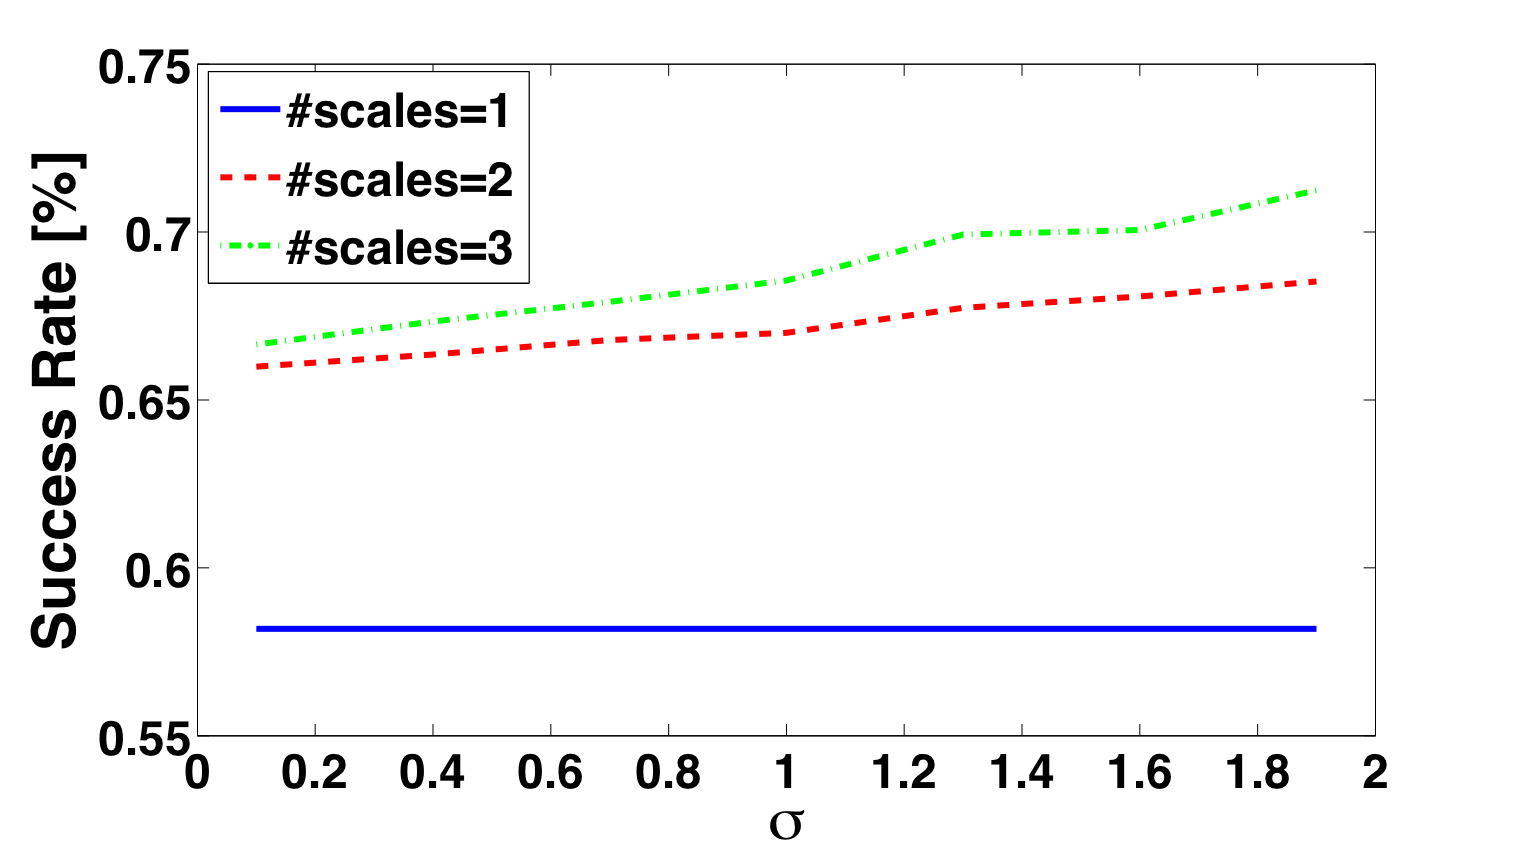
\includegraphics[width=3in]{figures_pami/multiscale.png}
\vspace{-2mm}
\caption{{\bf Multiscale alignment.} This figure shows the average success rate of alignment over all possible perturbations. A smaller blur kernel can be applied to achieve certain level of performance when more scales are used.}
\label{fig:multiscale}
\vspace{-4mm}
\end{figure}

\noindent{3) \em 3D Pose Variation.} As densely sampled pose
and
    illumination face images are not available in any of
    the public databases, including Multi-PIE, we have
    collected our own dataset using our own system (to be
    introduced in the next section). We use frontal face
    images of a subject under the 38 illuminations proposed
    in the next section as training. For testing, we
    collect images of the subject under a typical indoor
    lighting condition at pose ranging from $-90^\circ$ to
    $+90^\circ$ with step size 5.625$^\circ$, a total of 33
    poses. We use Viola and Jones' face detector to
    initialize our alignment algorithm.
Figure \ref{fig:pose-alignment} shows that our algorithm works reasonably well with poses up
to $\pm 45^\circ$.
Note that this level of out-of-plane
 pose variation is beyond what we intend to handle with our formulation.
\begin{figure}
\centering
{\small
\begin{tabular}{ccccc}
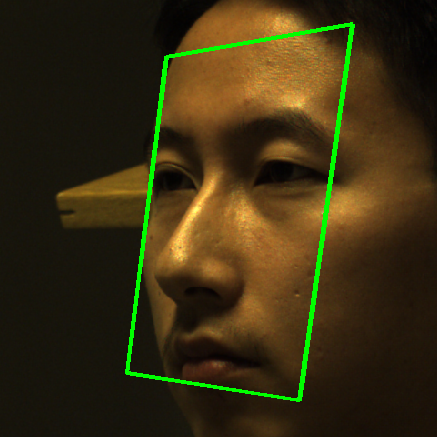
\includegraphics[height=0.5in]{figures_cvpr/5} &
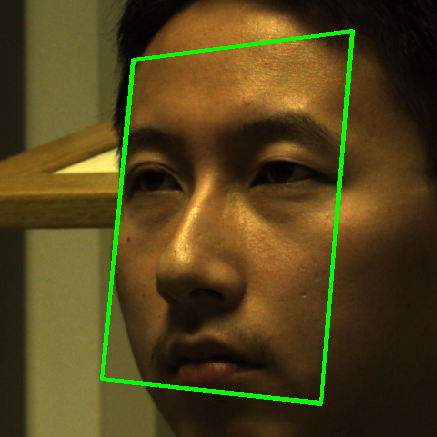
\includegraphics[height=0.5in]{figures_cvpr/7} &
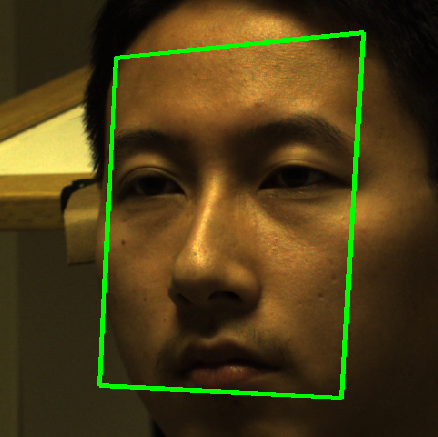
\includegraphics[height=0.5in]{figures_cvpr/09} &
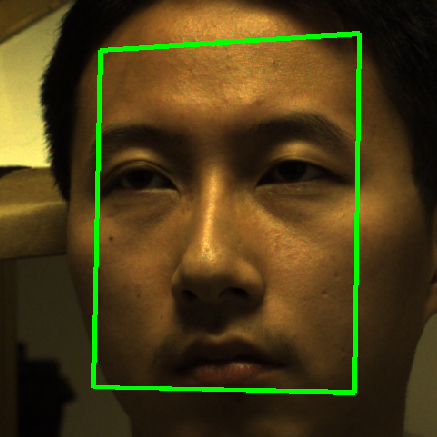
\includegraphics[height=0.5in]{figures_cvpr/11} &
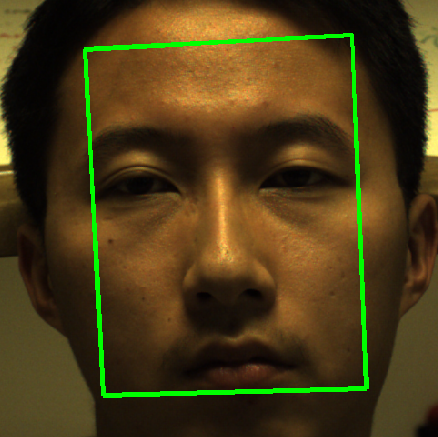
\includegraphics[height=0.5in]{figures_cvpr/13} \vspace{0mm} \\
(a) & (b) & (c) & (d) & (e)\\
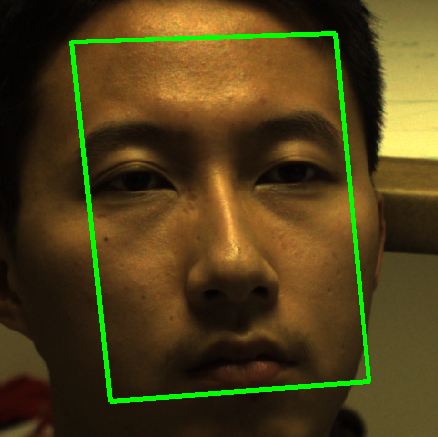
\includegraphics[height=0.5in]{figures_cvpr/15} &
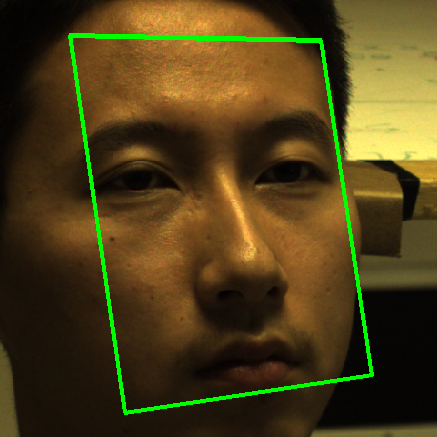
\includegraphics[height=0.5in]{figures_cvpr/17} &
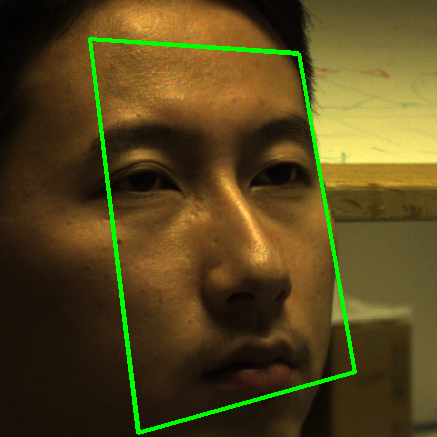
\includegraphics[height=0.5in]{figures_cvpr/19} &
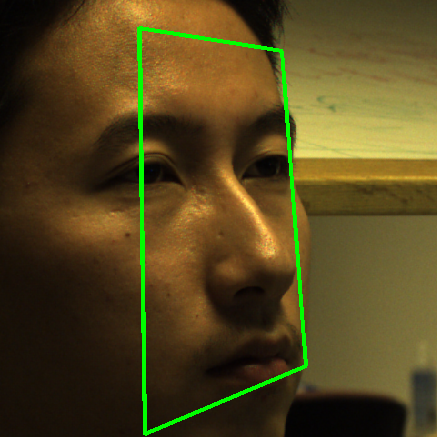
\includegraphics[height=0.5in]{figures_cvpr/21} &
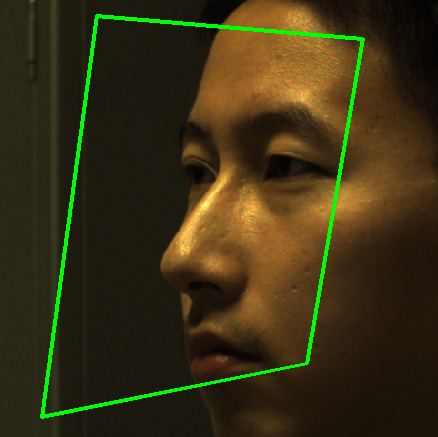
\includegraphics[height=0.5in]{figures_cvpr/3} \vspace{0mm} \\
(f) & (g) & (h) & (i) & (j) \vspace{0mm}
\end{tabular}
}
\caption{{\bf 2D Alignment of test images with different poses to frontal training images.} {\bf (a) to (i):}  plausible alignment for pose from $-45^{\circ}$
to $+45^{\circ}$. {\bf (j):} a case when the algorithm fails for an extreme pose ($>45^{\circ}$).
}\label{fig:pose-alignment} \vspace{-4mm}
\end{figure}
\subsection{Comparison with Related Work}
Our modification to SRC roots solidly in the tradition of
adding deformation-robustness to face recognition algorithms
\cite{Cootes2001-PAMI,Gross2006-PAMI,Wiskott1997-PAMI}.
However, the only previous work to investigate face alignment
in the context of sparse signal representation and SRC is the
work of \cite{Huang2008-CVPR}. They consider the case where the
training images themselves are misaligned and allow one
deformation per training image. They linearize the training
rather than the test, which is computationally more costly as
it effectively triples the size of the training set. In
addition, as they align the test image to all subjects
simultaneously, it potentially is more prone to local minima
when the number of subjects increases, as we will see in the
following experimental comparisons.
\begin{enumerate}
\item {\em Extended Yale B.} In this experiment, we have
    used the same experimental settings as in
    \cite{Huang2008-CVPR}. 20 subjects are selected and
    each has 32 frontal images (selected at random) as
    training and another 32 for testing. An artificial
    translation of 10 pixels (in both $x$ and $y$
    directions) is introduced to the test image. For our
    algorithm we downsample all the images to $88\times
    80$ for memory reasons, whereas the work of
    \cite{Huang2008-CVPR} uses random projections.
Note that the use of cropped images in this experiment introduces image boundary effects.
    Our
    algorithm achieves the recognition rate 93.7\%,
    compared to 89.1\% recognition rate reported in
    \cite{Huang2008-CVPR}.
\item {\em CMU Multi-PIE.} In this experiment, we choose
    all subjects from the CMU Multi-PIE database, 7
    training images from Session 1 and 1 test image from
    Session 2 per person. The setting is exactly the same
    as the previous experiment on 2D deformation. We again
    work with downsampled images of size $80\times 60$ pixels. An
    artificial translation of 5 pixels (in both $x$ and $y$
    directions) was induced in the test image. The
    algorithm of \cite{Huang2008-CVPR} achieves a
    recognition rate of 67.5\%,\footnote{That algorithm has
    two free parameters - $l$ and $d$, which govern the tradeoff between
	accuracy and run-time. For this experiment
    we chose $l = 1$ and $d = 514$.} while ours achieves 92.2\%.
    \end{enumerate}
				
\section{Handling Illumination Variation}\label{sec:illumination}
In the above section, we have made the assumption that the test image, although taken under some arbitrary illumination, can be linearly represented by a finite number of training illuminations.  Under what conditions is this a reasonable assumption to make?  What can we say from first principles about how the training images should be chosen?

\subsection{The Illumination Model}

The strongest theoretical results so far regarding the relationship
between illumination and the resulting sets of images is due to Basri and Jacobs \cite{Basri2003-PAMI}.
The main result of this paper is that for convex Lambertian objects, distant illuminations, and fixed pose,
all images of the object can be well approximated by linear combinations of
nine (properly chosen) basis images.  The basis images have mixed sign, and
their illuminations consist of the lowest frequency spherical harmonics.
While this is a very important result for understanding the image
formation process, the direct application of this result in most practical
systems is misguided for several reasons.
Specularities, self-shadowing, and inter-reflections all dramatically affect the appearance of face images,
and they all do so in a way that violates the modeling assumptions of the Basri analysis.

Fortunately, even with these effects, for most materials the relationship between
illumination and image is still linear,\footnote{Materials that break
this assumption include fluorescent materials and the photochromic (``Transition'') lenses
in some eyeglasses.  Most materials emit light in proportion to their
incident light.} provided the sensor has a linear response curve.\footnote{Proper handling of gamma encoding is an important consideration for
practitioners.  Most cameras apply a non-linear and often undocumented response
curve to captured images.  A slight degradation of performance will occur if
gamma compressed images are treated as if they were linear.  We recommend the use
of cameras with well documented response curves that can be inverted when the
image file is loaded.}
For a more in-depth study
of the relationship between illumination and images, we refer the reader to
\cite{belhumeur1998set}.
While the relationship between illuminations and images is linear,
only positive weights are allowed; the space of all images of an object with
fixed pose and varying illumination is a convex cone lying in the positive
orthant. The question becomes, how many images does it take to do a good job
of representing images sampled from this cone?

It has been observed in various empirical studies that
one can get away with using a small number of frontal
illuminations to linearly represent a wide range of new frontal
illuminations, when they are all taken under the same laboratory conditions
\cite{Georghiades2001-PAMI}. This is the case for many public
face datasets, including AR, ORL, PIE, and Multi-PIE.
Unfortunately, we have found that in practice, a training
database consisting purely of frontal illuminations is not
sufficient to linearly represent images of a faces taken
under typical indoor or outdoor conditions (see the experiment
conducted in Section \ref{sec:own-data}). As illustrated by the
example in Figure \ref{fig:promo}, an insufficient number of
training illuminations can result in recognition failure. To
ensure our algorithm works in practice, we need to find a set
of training illuminations that are indeed {\em sufficient} to
linearly represent a wide variety of practical indoor and
outdoor illuminations.


\subsection{Projector-based Illumination System}

We have designed a system that can acquire frontal images of a subject while
simultaneously illuminating the subject from all directions above horizontal. A sketch of the
system is shown in Figure \ref{fig:system}: The illumination
system consists of four projectors that display various bright
patterns onto the three white walls in the corner of a dark
room.  The light reflects off of the walls and illuminates the
user's head indirectly.  After taking the frontal illuminations
we rotate the chair by 180 degrees and take pictures from the
opposite direction.  Having two cameras speeds the process
since only the chair needs to be moved in between frontal and
rear illuminations. Our projector-based system has several
advantages over flash-based illumination systems for face recognition:
\begin{itemize}
\item The illuminations can be modified in software, rather than hardware.
\item It is easy to capture many different illuminations quickly.
\item Good coverage and distant illumination can be achieved simultaneously.
\item There is no need to mount anything on the walls or construct a large dome.
\item The system can be assembled from off-the-shelf hardware.
\end{itemize}
\begin{figure}
\centering
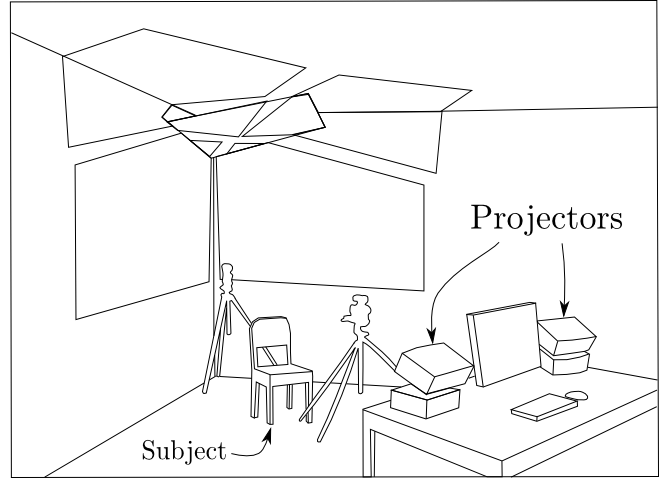
\includegraphics[height=2in]{figures_cvpr/camera_rig.pdf}
\caption{{\bf Training acquisition system:} Four projectors and two cameras controlled by one computer.}
\vspace{-2em}
\label{fig:system}
\end{figure}
With our projector system, our choice of illuminations is
constrained only by the need to achieve a good
SNR\footnote{Since illuminations with more pixels illuminated
will have a better SNR (provided they don't saturate), there is
an engineering tradeoff between the SNR and the number of
training images.}, avoid saturation, and achieve
a reasonably short acquisition time.  Two simplifying
assumptions that we make are that every pixel is either turned
fully on or off in every illumination, and that the illuminated
regions do not overlap.

Assuming that each pixel is fully on or off enables us to guarantee
that each illumination image has the same overall intensity, merely
by guaranteeing that we illuminate the same number of pixels in each image.\footnote{Since DLP projectors may have dramatically different response
curves depending on the mode they are in, it is not advisable to simply normalize each illumination image by its mean.}
Since our algorithm depends only on  the
linearity between the illuminations and the images, and not on the
relative intensities of the illuminations, the designer has the freedom to choose the overall intensity of the illuminations
to prevent saturation or low SNR, in a sort of offline exposure control.

Assuming that the sequentially illuminated regions do not overlap results in a
set of training images that span a larger cone than a similar number of
overlapping regions.  This results in training images that require fewer
negative coefficients in $\x$ to represent test images under natural
illuminations.  The effect of negative coefficients in $\x$ appears to depend
partly on how the test images are taken and is still under study.

{\em Relationship to existing work:} Most light stages used for face recognition have
been constructed for the purpose of creating public data sets to study
illumination invariance \cite{Georghiades2001-PAMI, Gross2008-FGR}.  Many other
light stages have been used for computer graphics purposes
\cite{debevec2000acquiring, jones2005performance}.
The light source can be
moved around manually \cite{masselus2002free}, but this may result in poor
consistency of illuminations between users.  Structured light applications use projectors to
directly illuminate the face (or other object) \cite{zhang2002rapid} for 3D
reconstruction, but this is very disturbing to the user.
Y.\ Schechner \cite{schechner2007multiplexing}
studies techniques for multiplexing illumination that can dramatically reduce the noise
of the demultiplexed images for certain classes of objects and cameras.
While these techniques have not been incorporated into the current
system, they fit elegantly into our framework and will likely be used
in future implementations.  We stress that use of this multiplexing technique
is independent from the choice of original (directional) illuminations.

\subsection{Choice of Illumination Patterns}

We ran two experiments to guide our choice of illuminations for
our large-scale experiments:
\begin{enumerate}
\item {\em Coverage Experiment.} In the first experiment we
    attempt to determine what coverage of the sphere is
    required to achieve good interpolation for test images.
    The subject was illuminated by 100 (50 front, 50 back)
    illuminations arranged in concentric rings centered at
    the front camera.  Subsets of the training images were
    chosen, starting at the front camera and adding a ring
    at a time.  Each time a ring was added to the training
    illumination set, the average $\ell^1$ registration
    error (residual) for a set of test images taken under
    sunlight was computed and plotted in Figure
    \ref{fig:illumination-patterns}(a).  The more rings of
    training illuminations are added, the lower the
    representation error becomes, with diminishing returns.
\item {\em Granularity Experiment.} In the second
    experiment we attempt to determine how finely divided
    the illumination sphere should be.  At the first
    granularity level, the projectors  illuminate the
    covered area uniformly.  At each subsequent granularity
    level each illuminated cell is divided in two along its
    longer side but intensity doubled.  For each
    granularity level the average $\ell^1$ registration
    error is computed as in the coverage experiment and
    shown in Figure \ref{fig:illumination-sufficiency}(b).
    Again, diminishing returns are observed as more
    illuminations are added.
\end{enumerate}
\begin{figure}
\centering
\begin{tabular}{cc}
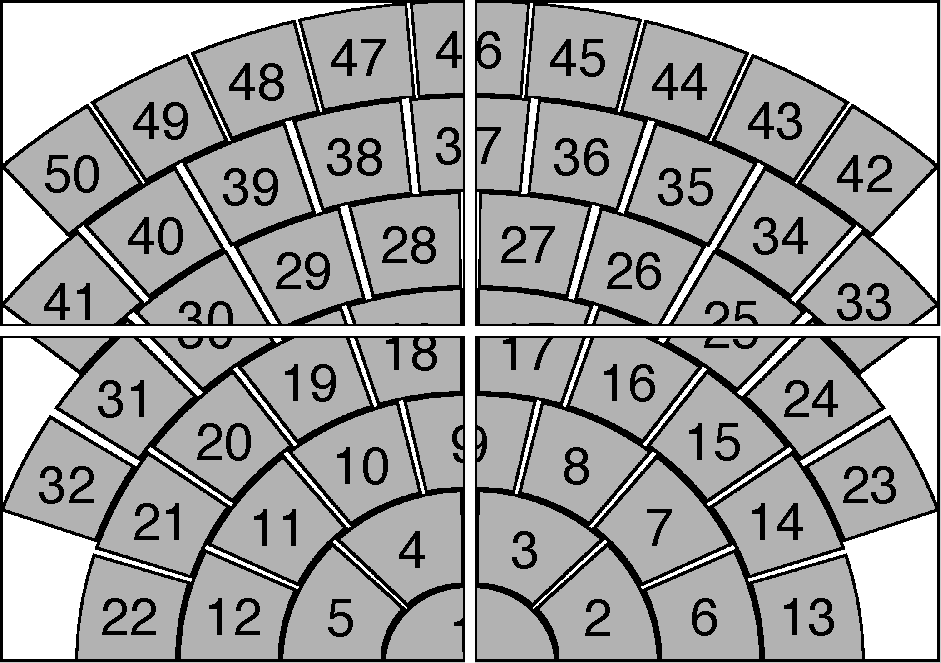
\includegraphics[height=.75in]{figures_cvpr/coverage_experiment_asplode.png} &
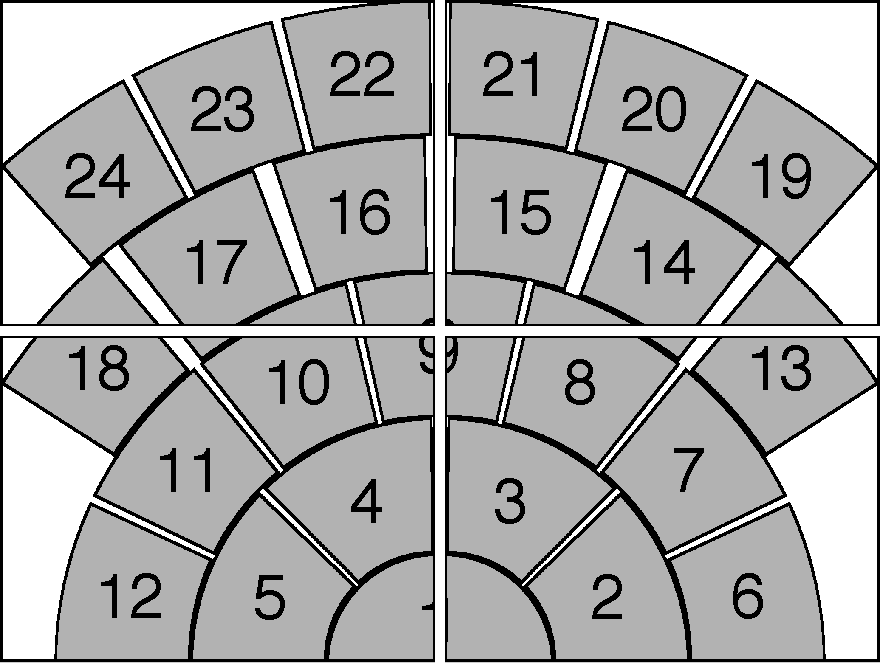
\includegraphics[height=.75in]{figures_cvpr/final_cvpr_illuminations_asplode.png}  \\
(a) Coverage Experiment & (b) Chosen Illumination Patterns
\end{tabular}\vspace{0mm}
\caption{{\bf Illumination Patterns.}   The cells are illuminated in sequence.  For rear illuminations the sequence is reversed.  In the chosen pattern's rear illumination, the cells 1-5 and 7-11 are omitted for a total of 38 illuminations. The four rectangular regions correspond to the four projectors.  }
\label{fig:illumination-patterns}
\vspace{-.75em}
\end{figure}

\begin{figure}
\centering
\begin{tabular}{@{}c@{}c@{}}
\includegraphics[height=1.2in]{figures_cvpr/illum_results/coverage_sunset.pdf} &
\includegraphics[height=1.2in]{figures_cvpr/illum_results/granularity_sunset.pdf} \\
(a) Coverage & (b) Granularity
\end{tabular}\vspace{0mm}
\caption{{\bf Study of sufficient illuminations.} The average $\ell^1$ registration residual versus different illumination training sets. }
\label{fig:illumination-sufficiency}
\vspace{-4.5em}
\end{figure}

In the plot for the coverage experiment, Figure
\ref{fig:illumination-sufficiency}(a),
 we clearly see two plateau regions: one is after 4 rings
and one is after 10 rings. The first four rings represent the
typical frontal illuminations, which are present in most public
face datasets; however, we see that the residual stabilizes
after 10 rings which include some illuminations from the back
of the subject. This suggests that although the frontal
illuminations account for most of the illumination on the face,
some illuminations from the back are needed in the training set to
represent images with illumination coming from all directions.
In the plot for the granularity experiment, Figure
\ref{fig:illumination-sufficiency}(b), we observe that the
residual reaches a plateau after four divisions, corresponding
to a total of 32 illuminations. Based on the results from both
experiments, we decide to partition the area covered by the
first 10 rings into a total of 38 cells, whose layout is
explained in Figure \ref{fig:illumination-patterns}(b). For
our large-scale experiments, we have collected those
illuminations for all our subjects.\footnote{It is possible
that with further experimentation a reduced set of illuminations
can be found that performs as well or better.}

See below for the 38 training images of one subject:
\begin{figure}[h]
\centering
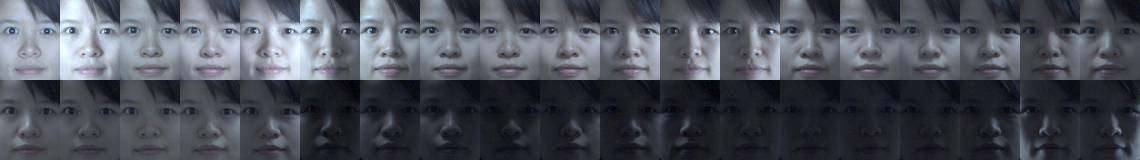
\includegraphics[width=3.2in]{figures_cvpr/training.png}
\vspace{-2em}
\end{figure}

\section{Tests on Public Databases}\label{sec:multipie}
In this section and the next section, we conduct comprehensive experiments on
large-scale face databases to verify the performance of our algorithm and
system. We first test on the largest public face database available that is
suitable for testing our algorithm, the CMU Multi-PIE.  One shortcoming of the
CMU Multi-PIE database for our purposes is that there is no separate set of
test images taken under natural illuminations; we are left to choose which sets
of images to use for testing and training.  To challenge our algorithm, we
choose only a small set of illuminations for the training set, yet we include
all illuminations in the testing set. In the following section, we will test
our algorithm on a face dataset that is collected by our own system. The goal
for that experiment will be to show that with a sufficient set of training
illuminations for each subject, our algorithm indeed works stably and robustly
with practical illumination, misalignment, pose, and occlusion, as already
indicated by our experiment shown in Figure \ref{fig:promo}(bottom).

CMU Multi-PIE provides the most extensive test set among public
datasets. This database contains images of 337 subjects across
simultaneous variation in pose, expression, and illumination.
Of these 337 subjects, we use all of the 249 subjects present
in Session 1 as the training set. The remaining 88 subjects are
treated as ``impostors'', or invalid images. For each of the
249 training subjects, we include frontal images of 7 frontal
illuminations,\footnote{They are illuminations
$\{0,1,7,13,14,16,18\}$ of \cite{Gross2008-FGR}. For each
directional illumination, we subtract the ambient-illuminated
image 0.} taken with neutral expression. As suggested by the
work of \cite{Georghiades2001-PAMI}, we choose these extreme
frontal illuminations in the hope that they would linearly
represent other frontal illuminations well. For the test set,
we use all 20 illuminations from Sessions 2-4, which were
recorded over a period of several months. The dataset is
challenging due to the large number of subjects, and due to
natural variation in subject appearance over time.
Table \ref{tab:MultiPIE-recognition2} shows the result of our
algorithm on each of the 3 testing sessions. Our algorithm
achieves recognition rates above $90\%$ for all three sessions.
For the test images, our iterative alignment was initialized
automatically via the Viola and Jones' face detector. To
demonstrate that the sparse representation based recognition
step is indeed beneficial even when there are no impostors, we
include results for recognition based only on the alignment
error residuals (i.e. $S=1$), shown in row 1.

\begin{table}
\caption{Recognition rates on the Multi-PIE database for
Algorithm 1 and \cite{Yang2010-CVPR}}
\centerline{
\begin{tabular}{|c|c|c|c|c| }
\hline
Recognition rate & Session 2 & Session 3 & Session 4  \\
\hline
{Alg. 1, $S=1$} & 90.7\% & 89.6\% & 87.5\% \\
\hline
{Alg. 1} & 93.9\% & 93.8\% & 92.3\% \\
\hline
{Alg. 1 with improved window} & 95.0\% & {\bf 96.3}\% & {\bf 97.3}\% \\
\hline
\cite{Yang2010-CVPR} & {\bf 95.2}\% & 93.4\% & 95.1\% \\
\hline
\end{tabular}
\label{tab:MultiPIE-recognition2} }
\end{table}

\newcommand{\tempwidth}[0]{0.58in}
\begin{figure}
\centering
{\small
\begin{tabular}{@{}c@{}c@{}c@{}c@{}c@{}c@{}}
\hspace{-2mm}
\includegraphics[width=\tempwidth,clip=true]{figures_pami/multipie_failed/079_01_01_051_08.png}  &
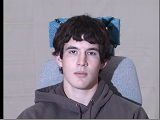
\includegraphics[width=\tempwidth,clip=true]{figures_pami/multipie_failed/111_01_01_051_08.png}  &
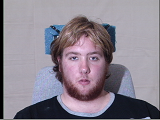
\includegraphics[width=\tempwidth,clip=true]{figures_pami/multipie_failed/196_01_01_051_08.png}  &
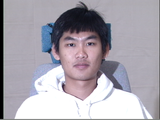
\includegraphics[width=\tempwidth,clip=true]{figures_pami/multipie_failed/130_01_01_051_08.png}  &
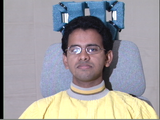
\includegraphics[width=\tempwidth,clip=true]{figures_pami/multipie_failed/163_01_01_051_08.png}  &
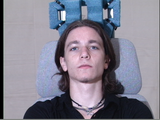
\includegraphics[width=\tempwidth,clip=true]{figures_pami/multipie_failed/175_01_01_051_08.png} \\
\hspace{-2mm}
\includegraphics[width=\tempwidth,clip=true]{figures_pami/multipie_failed/079_02_01_051_08.png}  &
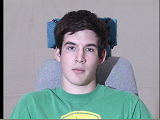
\includegraphics[width=\tempwidth,clip=true]{figures_pami/multipie_failed/111_02_01_051_08.png}  &
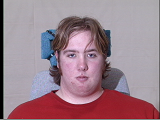
\includegraphics[width=\tempwidth,clip=true]{figures_pami/multipie_failed/196_02_01_051_08.png}  &
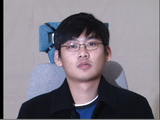
\includegraphics[width=\tempwidth,clip=true]{figures_pami/multipie_failed/130_02_01_051_08.png}  &
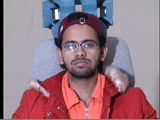
\includegraphics[width=\tempwidth,clip=true]{figures_pami/multipie_failed/163_02_01_051_08.png}  &

\includegraphics[width=\tempwidth,clip=true]{figures_pami/multipie_failed/175_02_01_051_08.png} \\
\hspace{-2mm}(a) & (b) & (c) & (d) & (e) & (f) \vspace{0mm}
\end{tabular}
}
\caption{{\bf Representative failures from Multi-PIE}. {\bf Top:} training from Session 1; {\bf Bottom:} test images from Session 2. Due to changes in hair, glasses, beard, or pose, our alignment fails on these subjects regardless of test image illumination.}
\label{fig:failed-examples}
\vspace{-4mm}
\end{figure}

\subsection{Improving the Sampling Window}
Our algorithm's errors are mostly caused by a few subjects who
significantly change their appearances between sessions (such
as hair, facial hair, and eyeglasses). Some representative
examples are shown in Figure \ref{fig:failed-examples}. For those subjects, alignment and recognition fail on
almost all test illuminations.

Meanwhile, this observation also suggests that we might be able
to improve the performance of our method by carefully choosing
a face region which is less affected by the above factors for
recognition. In particular, since the forehead region is likely
to be affected by the change of hair style, we try replacing
the previous $80 \times 60$ canonical frame with a new
window that better excludes the forehead. We adjust the
resolution of the window to keep $m$ approximately constant. In addition,
we cut off two lower corners of the $80 \times 60$ canonical frame, motivated by
the observation that in many cases the corners
actually contain background. An example of the new window
is shown in Figure~\ref{fig:new-mask}.

\begin{figure}
\vspace{-1em}
\centering
{\small
\begin{tabular}{@{}cc@{}}
\includegraphics[trim=1.9in .7in 1.9in .5in, clip, height=1.0in]{figures_pami/example.png} &
\includegraphics[trim=1.9in .7in 1.9in .5in, clip, height=1.0in]{figures_pami/example_new.png} \vspace{0mm} \\
Default window. & Proposed window. \vspace{0mm}
\end{tabular}
}
\caption{{\bf Choosing different sampling windows.}}
\label{fig:new-mask}
\vspace{-1em}
\end{figure}

Table \ref{tab:MultiPIE-recognition2} shows that the
recognition rates on Multi-PIE indeed increase with this new
window. In addition, Figure \ref{fig:failed-examples}(a), (b),
and (c) illustrate three representative subjects for which the
recognition rates of our algorithm are significantly boosted
with the new window. However, we should mention that the best
choice of the window is problem-specific and there is not a
simple guideline to follow. For example, although the new
window performs better on Multi-PIE, the same window does not
help at all on our own database, which will be introduced in
the next section. This is because most of the training and
testing images in our database are taken on the same day so the
variation in hair style is very small. Hence, excluding the
forehead part may actually result in loss of useful
discriminative information.

\subsection{Comparison to Existing Work}
We first compare our result to the recent work
\cite{Yang2010-CVPR}. Notice that in \cite{Yang2010-CVPR}, the
initial registration is obtained from manually selected outer
eye corners. Then, a supervised hierarchical sparse coding
model based on local image descriptors is trained, which enjoys
certain translation invariant properties. With the same
training and testing sets, \cite{Yang2010-CVPR} is able to
handle the remaining misalignment and achieves state-of-the-art
performance on the CMU Multi-PIE database.
Table~\ref{tab:MultiPIE-recognition2} shows that our algorithm
achieves similar or better performance on different sessions of
Multi-PIE.

% Classical algorithms
To better examine the effectiveness of our iterative alignment
algorithm, we next compare our result to baseline
linear-projection-based algorithms, such as Nearest Neighbor
(NN), Nearest Subspace (NS) \cite{Lee2005-PAMI}, and Linear
Discriminant Analysis (LDA)
\cite{Belhumeur1997-PAMI}.\footnote{We do not list results on
PCA \cite{Turk1991-CVPR} as its performance is always below
that of Nearest Subspace.} Since these algorithms assume
pixel-accurate alignment, they are not expected to work well if
the test image is not well aligned with the training. In
Table~\ref{tab:MultiPIE-recognition}, we report the results of
these classical algorithms with three types of testing image
alignment: 1.\ alignment from the Viola and Jones' detector,
2.\ alignment via manually selected outer eye
corners,\footnote{Two manually clicked points are sufficient to
define a similarity transformation. All of the experiments in
this section are carried out with similarity transformations.}
and 3.\ the output of our iterative alignment algorithm. The
performance drop of the LDA algorithm on Multi-PIE reported
here seems to agree with that reported already in
\cite{Gross2008-FGR}.  All of the classical algorithms benefit
greatly from being paired with our iterative alignment
algorithm.

\begin{table*}
\centering
\caption{Recognition rates on the Multi-PIE database for
different pairings of alignment and recognition stages.}
\centerline{
\begin{tabular}{|c|c|c|c|c|c|c|c|c|c|c| }
\hline
\backslashbox{Rec.}{Align.}
& \multicolumn{3}{|c|}{Face Detector}
& \multicolumn{3}{|c|}{Manual}
& \multicolumn{3}{|c|}{Iterative Alignment}
\\
\hline
Session $\rightarrow$	& 2		&3			&4			& 2		&3			&4			& 2		&3			&4		\\
\hline
NS	& 30.8\%	& 29.4\%	& 24.6\%	& 77.6\%	& 74.3\%	& 73.4\%	& 84.5\%	& 82.3\%	& 81.4\% \\
\hline
NN	& 26.4\%	& 24.7\%	& 21.9\%	& 67.3\%	& 66.2\%	& 62.8\%	& 73.5\%	& 69.6\%	& 69.3\% \\
\hline
LDA	& 5.1\%		& 5.9\%		& 4.3\%		& 49.4\%	& 44.3\%	& 47.9\%	& 91.0\%	& 89.9\%	& 88.1\% \\
\hline
LBP	& 39.9\%	& 38.1\%	& 33.9\%	& 93.3\%	& 91.2\%	& 92.9\%	& {\bf 95.2\%}	& {\bf 94.7\%}	& {\bf 93.5\%} \\
\hline
SRC	& -- & -- & -- & -- & -- & -- & 93.9\%	& 93.8\%	& 92.3\% \\
\hline
\end{tabular}
\label{tab:MultiPIE-recognition} }
\vspace{-.1in}
\end{table*}

% LBP
We also compare our result to Local Binary Patterns (LBP)
\cite{Ahonen2006-PAMI}, a local appearance descriptor which is
able to capture fine details of facial appearance and texture.
Due to its robustness to variations in illumination, facial
expression, aging and other changes, LBP has achieved the
state-of-the-art face recognition performance in the scenario
when only one sample per person is used for training
\cite{Tan06facerecognition}.
In this paper, we follow the same
steps as in \cite{Ahonen2006-PAMI} to construct an LBP
descriptor for each training and testing sample. The $80\times
60$ face region is first divided into a regular $10\times 10$
grid of cells, each of size $8\times 6$ pixels. Within each
cell, the histogram of 59 uniform binary patterns is then
computed, where the patterns are generated by thresholding 8
neighboring pixels in a circle of radius 2 using the central
pixel value. Finally, the local histograms are concatenated to
produce the global descriptor vector. As suggested in
\cite{Ahonen2006-PAMI}, the recognition is performed using a
nearest neighbor classifier with Chi square distance as the
distance measure and we report the recognition rates with the
same three types of input as before.  As shown in
Table~\ref{tab:MultiPIE-recognition}, although LBP achieves
competitive recognition rates given manually aligned training
and testing samples, demonstrating its robustness to moderate
misalignment, it still benefits from using the output of our
iterative alignment algorithm as the input.
In addition, like
the other classical algorithms, the performance of LBP degrades
dramatically if it is applied directly to the output of a face
detector. This is notable given that LBP is often applied
without any special alignment in practice. Finally, we
attribute the improvement in performance of LBP over SRC in
this experiment to its robustness to illumination components
that cannot be linearly interpolated by the training set.

In addition, although our algorithm is not designed for
recognition when there is only a single gallery image per user,
we compare its performance with LBP within this setting for
completeness. For this experiment, we use the FERET dataset
\cite{phillips1998feret}, which contains five standard
partitions: `fa' is the gallery containing 1196 frontal images
of 1196 subjects, and `fb', `fc', `dup1' and `dup2' are four
sets of probe images. The testing sets differ from the training
in facial expression (`fb'), illumination (`fc'), aging (`dup1'
) and long aging (`dup2'). In fact, except for `fb', we notice
significant changes of illumination in all the other three test
sets. For the training, we again crop and normalize the face
region from each original image to an $80\times 60$ window
using manually marked eye coordinates \cite{Deng2010-PR}. In
Table~\ref{tab:FERET-recognition}, we report the performance of
our algorithm on the four test sets, with input directly
obtained from the Viola and Jones' detector. We also report the
performance of LBP with the same three types of input as before:
we use letters
``$d$'', ``$m$'', and ``$i$'' to indicate face detector, manual
alignment, and our iterative alignment algorithm, respectively.

\begin{table}
\caption{Performance on single gallery image FERET dataset}
\vspace{-3mm} \centerline{
\begin{tabular}{|c|c|c|c|c| }
\hline
Recognition rate \% & fb & fc & dup1 & dup2 \\
\hline
$LBP_d$ & 54.8 & 10.3 & 29.8 & 19.8 \\
\hline
$LBP_m$ & {\bf 96.6} & {\bf 58.8} & {\bf 71.6} & {\bf 61.5} \\
\hline
$LBP_i$ & 94.5 & 42.8 & 46.5 & 21.1 \\
\hline
{Alg. 1} & 95.2 & 28.4 & 46.1 & 20.3 \\
\hline
\end{tabular}
\label{tab:FERET-recognition} }
\vspace{-12mm}
\end{table}

As expected, our algorithm does not perform well except for
`fb', in which the illumination is similar to the training and
the mere variation in facial expression is handled well by the
sparse error model. For the other three test sets, our
algorithm fails because the illumination changes and other
variations seriously violate the assumptions of our method.
This also explains why LBP performs worse with our iterative
alignment algorithm, compared to manual alignment. On the other
hand, while LBP achieves the best recognition rates given
manually aligned training and testing samples, its performance
degrades drastically when the input is obtained directly from
the face detector. It is also worth noting that similar poor
performance of LBP, as well as other descriptors, has been
observed on the Labeled Face in the Wild (LFW) database, where
the training is uncontrolled and limited and the input is
directly obtained from the face detector \cite{Wolf2008-ECCV}.

All of these experimental results confirm that
both illumination and alignment need to be simultaneously handled
well in order to achieve accurate face recognition, even when there is
no obvious occlusion or corruption in the test.

\subsection{Subject Validation}

We test the algorithms' ability to reject invalid images of the
88 subjects not appearing in the training database. As
mentioned before, the \emph{sparsity concentration index} (SCI)
is used as the outlier rejection rule. Given the sparse
representation $\x$ of a test image with respect to $K$
training classes, the SCI measures how concentrated the
coefficients are on a single class in the dataset and is
defined as in \cite{Wright2009-PAMI}:
\begin{displaymath}
\textup{SCI}(\x) \doteq \frac{K \cdot \max_i \|\delta_i(\x)\|_1 /
\|\x\|_1 - 1}{K - 1} \in [0,1] .
\end{displaymath}
It is easy to see that if $\textup{SCI}(\x) = 1$, the test
image is represented using images from one single subject
class; if $\textup{SCI}(\x) = 0$, the coefficients are spread
evenly over all classes. Thus, we can choose a threshold $t \in
[0,1]$ for the proposed method and accept a test image as valid
if $\textup{SCI}(\x) \geq t$, and otherwise reject it as
invalid. We compare this classifier to classifiers based on
thresholding the error residuals of NN, NS, LDA, and LBP.
\begin{figure}[t]
{\small
\centering
\begin{tabular}{@{}c@{}c@{}}
\includegraphics[height = 1.6in]{figures_pami/pami_roc_revision2} & \hspace{2mm}
\includegraphics[height = 1.6in]{figures_pami/pami_roc2} \\
(a) & \hspace{2mm}(b) \\
\end{tabular}
}
\vspace{-2mm}
\caption{{\bf ROC curves} for subject validation on Multi-PIE database,
(a) for all algorithms with iterative alignment, and
(b) for the classical algorithms with manual alignment (indicated by a subscript ``m'').}\label{fig:roc-multipie}
\vspace{-2mm}
\end{figure}

Figure \ref{fig:roc-multipie} plots the receiver operating
characteristic (ROC) curves, which are generated by sweeping
the threshold $t$ through the entire range of possible values
for each algorithm.\footnote{Rejecting invalid images not in
the entire database is much more difficult than deciding if two
face images are the same subject. Figure \ref{fig:roc-multipie}
should not be confused with typical ROC curves for face
similarity, e.g., \cite{PhillipsP2007}.} On the left we can see
that the SCI based recognition approach significantly
outperforms the other algorithms, including LBP, even when all
algorithms are coupled with our proposed iterative alignment.
In the right plot we again see that classical algorithms, and
even LBP, are very sensitive to alignment.  Similar contrasts
between our algorithm and baseline algorithms were also
observed for SRC in \cite{Wright2009-PAMI}, though on much
smaller datasets.

\subsection{Recognition with Synthetic Random Block Occlusion}

We further test the robustness of our $\ell^1$-norm based
algorithm to synthetic occlusion. We simulate various levels of
occlusion from 10\% to 50\% by replacing a randomly located
block of the face image with an image of a baboon, as shown in
Figure~\ref{fig:multipie-occ-rec}. In this experiment, to avoid
any other factors that may contribute to extra occlusion of the
face (such as the change of hair style), we choose illumination
10 from Session 1\footnote{This is the same session as the
training set.} as testing. The rest of the experimental setting
remains unchanged. The table in
Figure~\ref{fig:multipie-occ-rec} shows that our algorithm is
indeed capable of handling a moderate amount of occlusion. For
example, at 20\% occlusion, our algorithm still achieves 94.9\%
recognition rate.

\newcommand{\tempscale}{0.40}
\begin{figure}
\centering
\begin{tabular}{@{}c@{}c@{}c@{}c@{}c@{}}
\includegraphics[scale=\tempscale,clip=true]{figures_pami/multipie_occ/occ10.png} &
\includegraphics[scale=\tempscale,clip=true]{figures_pami/multipie_occ/occ20.png} &
\includegraphics[scale=\tempscale,clip=true]{figures_pami/multipie_occ/occ30.png} &
\includegraphics[scale=\tempscale,clip=true]{figures_pami/multipie_occ/occ40.png} &
\includegraphics[scale=\tempscale,clip=true]{figures_pami/multipie_occ/occ50.png}  \\
\end{tabular}
\vspace{-1mm}
\caption{{\bf Recognition under varying level of
random block occlusion.} The above row shows examples of occluded test images with occlusion level from 10\% to 50\%. Our method maintains high recognition rates up to 30\% occlusion:}
\vspace{2mm}
{\small
\begin{tabular}{|c|c|c|c|c|c| }
\hline
Percent occluded & 10\% & 20\% & 30\% & 40\% & 50\%  \\
\hline
Recognition rate & 99.6\% & 94.9\% & 79.6\% & 46.5\% & 19.8\% \\
\hline
\end{tabular}
}
\label{fig:multipie-occ-rec}
\vspace{-.5in}
\end{figure}

\subsection{Recognition with Pose and Expression} We now run tests of
our algorithm on a subset of the images from Multi-PIE with pose and expression variation in the test set, although we do not model these variations explicitly.
Using the same training set as above, we test our algorithm on
images in Session 2 with $15^\circ$ pose, for all 20
illuminations. As expected, the recognition rate drops to 78.0\%. We also test our
algorithm on images in Session 3 with smile, again for all 20
illuminations. The recognition rate is 64.8\%. Of course, it is reasonable to expect that
the performance of our method will be significantly improved if pose and expression data
are available in the training.


%\vspace{-.1in}
\section{Tests on Our Own Database}\label{sec:own-data} Using the training acquisition
system we described in Section \ref{sec:illumination}, and shown in Figure
\ref{fig:system}, we have collected the frontal view of 109
subjects {\em without eyeglasses} under 38 illuminations shown
in Figure \ref{fig:illumination-patterns}. For testing our
algorithm, we have also taken 935 images of these subjects with
a different camera under a variety of practical conditions.
\vspace{-.1in}

\subsection{Necessity of Rear Illuminations} To see how
training illuminations affect the performance of our algorithm
in practice, we now compare how well a few frontal
illuminations can linearly represent: 1. other frontal illuminations
taken under the same laboratory conditions, and 2. typical
indoor and outdoor illuminations. To this end, we use the face
database acquired by our system and use 7 illuminations per
subject as training. The illuminations are chosen to be similar
to the 7 illuminations used in the previous experiment on
Multi-PIE.\footnote{We use the illuminations $\{6, 9, 12,
13, 18, 21, 22\}$ shown in Figure
\ref{fig:illumination-patterns}(b) to mimic the illuminations
 $\{0, 1, 6, 7, 13, 14, 18\}$ in Multi-PIE.} We then test
our algorithm on the remaining $24 - 7 = 17$ frontal
illuminations for all the subjects. The recognition rate is
$99.8\%$, nearly perfect. We also test our algorithm on 310
indoor images and 168 outdoor images of these subjects taken
under a variety of lighting conditions (category 1 and 2
specified below), similar to the one shown in Figure
\ref{fig:promo}, and the recognition rates for indoor and
outdoor images drop down to $94.2\%$ and $89.2\%$,
respectively. This is a strong indication that
frontal illuminations taken under laboratory conditions
are insufficient for representing test images under typical indoor and
outdoor illuminations.
\vspace{-0.1in}

\renewcommand{\tempscale}{0.45}
\begin{figure}
\centering
\begin{tabular}{@{}c@{}c@{}c@{}c@{}c@{}c@{}}
\includegraphics[scale=\tempscale,clip=true]{figures_pami/uiuc_example/normal_indoor/DSC_1318.JPG} &
\includegraphics[scale=\tempscale,clip=true]{figures_pami/uiuc_example/normal_indoor/DSC_1521.JPG} &
\includegraphics[scale=\tempscale,clip=true]{figures_pami/uiuc_example/normal_indoor/DSC_1673.JPG} &
\includegraphics[scale=\tempscale,clip=true]{figures_pami/uiuc_example/normal_indoor/DSC_1732.JPG} &
\includegraphics[scale=\tempscale,clip=true]{figures_pami/uiuc_example/normal_indoor/DSC_1941.JPG} &
\includegraphics[scale=\tempscale,clip=true]{figures_pami/uiuc_example/normal_indoor/DSC_3766.JPG} \\
\includegraphics[scale=\tempscale,clip=true]{figures_pami/uiuc_example/normal_outdoor/DSC_1574.JPG} &
\includegraphics[scale=\tempscale,clip=true]{figures_pami/uiuc_example/normal_outdoor/DSC_1622.JPG} &
\includegraphics[scale=\tempscale,clip=true]{figures_pami/uiuc_example/normal_outdoor/DSC_1641.JPG} &
\includegraphics[scale=\tempscale,clip=true]{figures_pami/uiuc_example/normal_outdoor/DSC_3522.JPG} &
\includegraphics[scale=\tempscale,clip=true]{figures_pami/uiuc_example/normal_outdoor/DSC_3707.JPG} &
\includegraphics[scale=\tempscale,clip=true]{figures_pami/uiuc_example/normal_outdoor/DSC_3772.JPG} \\
\includegraphics[scale=\tempscale,clip=true]{figures_pami/uiuc_example/glasses/DSC_1397.JPG} &
\includegraphics[scale=\tempscale,clip=true]{figures_pami/uiuc_example/glasses/DSC_1532.JPG} &
\includegraphics[scale=\tempscale,clip=true]{figures_pami/uiuc_example/glasses/DSC_1556.JPG} &
\includegraphics[scale=\tempscale,clip=true]{figures_pami/uiuc_example/glasses/DSC_1585.JPG} &
\includegraphics[scale=\tempscale,clip=true]{figures_pami/uiuc_example/glasses/DSC_1688.JPG} &
\includegraphics[scale=\tempscale,clip=true]{figures_pami/uiuc_example/glasses/DSC_4035.JPG} \\
\end{tabular}
\caption{{\bf Representative examples of categories C1-C3}. One row for each category.}\label{fig:examples1-3}
\vspace{-.1in}
\end{figure}

\begin{figure}[t]
\centering
\begin{tabular}{@{}c@{}c@{}c@{}c@{}c@{}c@{}}
\includegraphics[scale=\tempscale,clip=true]{figures_pami/uiuc_example/sunglasses/DSC_1565.JPG} &
\includegraphics[scale=\tempscale,clip=true]{figures_pami/uiuc_example/sunglasses/DSC_3656.JPG} &
\includegraphics[scale=\tempscale,clip=true]{figures_pami/uiuc_example/sunglasses/DSC_3827.JPG} &
\includegraphics[scale=\tempscale,clip=true]{figures_pami/uiuc_example/sunglasses/DSC_4090.JPG} &
\includegraphics[scale=\tempscale,clip=true]{figures_pami/uiuc_example/sunglasses/DSC_4106.JPG} &
\includegraphics[scale=\tempscale,clip=true]{figures_pami/uiuc_example/sunglasses/DSC_4126.JPG} \\
\includegraphics[scale=\tempscale,clip=true]{figures_pami/uiuc_example/sunglasses_failed/DSC_1611.JPG} &
\includegraphics[scale=\tempscale,clip=true]{figures_pami/uiuc_example/sunglasses_failed/DSC_3528.JPG} &
\includegraphics[scale=\tempscale,clip=true]{figures_pami/uiuc_example/sunglasses_failed/DSC_3744.JPG} &
\includegraphics[scale=\tempscale,clip=true]{figures_pami/uiuc_example/sunglasses_failed/DSC_3995.JPG} &
\includegraphics[scale=\tempscale,clip=true]{figures_pami/uiuc_example/sunglasses_failed/DSC_4030.JPG} &
\includegraphics[scale=\tempscale,clip=true]{figures_pami/uiuc_example/sunglasses_failed/DSC_4095.JPG} \\
\end{tabular}
 \caption{{\bf Representative examples of category C4}. Top row: successful examples with our method using overlapping blocks. Bottom row: failures with our method using overlapping blocks.}\label{fig:examples4}
\vspace{-.55in}
\end{figure}

\subsection{Large-Scale Test with Sufficient Training
Illuminations} Now we use all 109 subjects and 38 illuminations
in the training and test on 935 images taken under a variety of
practical illuminations and conditions. We have manually partitioned the test images into four main
categories:
\begin{description}
\item[C1:] 310 \emph{indoor} images of 72 subjects without
    eyeglasses, frontal view
    (Fig.~\ref{fig:examples1-3}, row 1).
\item[C2:] 168 \emph{outdoor} images of 48 subjects without
    eyeglasses, frontal view
    (Fig.~\ref{fig:examples1-3}, row 2).
\item[C3:] 211 images of 32 subjects with \emph{eyeglasses}
    (Fig.~\ref{fig:examples1-3}, row 3).
\item[C4:] 246 images of 56 subjects with \emph{sunglasses}
    (Fig.~\ref{fig:examples4}).
\end{description}
We apply Viola and Jones' face detector on these images and
directly use the detected faces as the input to our algorithm.
Table~\ref{tab:UIUC-recognition} reports the performance of our
algorithm on each category.
Since our focus is on face
recognition, the errors do not include failures of the face
detector on some of the more challenging images.
As one can see, our algorithm achieves higher than 95\%
recognition rates on categories 1-3. Furthermore, using the
full set of 38 illuminations indeed improves the performance of
our system under practical illumination conditions compared to
only using a small subset of 7 illuminations. However, the
performance dramatically drops when the faces are occluded by
various types of sunglasses, which could cover up to 40\% of
the entire face. Given the previous experimental results on
synthetic random block occlusions, and given that the
illuminations are more challenging, the result is not
surprising. In the next subsection, we will show how additional
assumptions can be used to improve the recognition performance.
\begin{table}[h]
\vspace{0mm}
\centering \caption{Recognition rates on our own
database.} \vspace{0mm}
\begin{tabular}{|c|c|c|c|c| }
\hline
Test Category & C1 & C2 & C3 & C4  \\
\hline
\hline
Recognition Rate & 98.4\% & 95.8\% & 95.1\% & 40.9\% \\
\hline
\end{tabular}
\label{tab:UIUC-recognition}
\vspace{0mm}
\end{table}

\subsection{Improving the Performance with Occlusion using Overlapping Blocks}
A traditional approach to improve the performance of face
recognition under severe occlusion is to use subregions instead
the entire face as a whole. This idea has been explored in many
earlier works; see \cite{Pentland1994-CVPR, Wright2009-PAMI}
for examples. Since in most real world cases the occlusion is contiguous, it is reasonable to argue that a minority of the
subregions are likely to be affected by the occlusion. In this
paper, we adopt the same idea and partition the face into four
overlapping blocks to better handle sunglasses. This
scheme is illustrated in Figure~\ref{fig:occ-block}. Notice
that in this example three out of the four blocks are partially
or almost completely occluded. In our experiment, each block is
of size $90\times 48$ and covers about two-fifths of the entire
face. The testing and training sets are partitioned in the same
way. We then independently apply
Algorithm~\ref{alg:deformable-src} and compute a sparse
representation after registration for each block independently
with respect to the training set. The recognition
results for individual blocks are then aggregated by voting.

\begin{figure}
\centering
\includegraphics[width=2.6in]{figures_pami/occ_block.png}
\caption{{\bf Using overlapping blocks to tackle contiguous occlusion.} (a) The test image, occluded by sunglasses. (b) The four overlapping blocks. (c) The sparse representation is calculated after alignment for each block independently. The red lines correspond to his true identity. (d) The true identity is successfully recovered by voting based on the SCI scores.}
\label{fig:occ-block}
\vspace{0mm}
\end{figure}

In this experiment, we found that the using the \emph{sparsity
concentration index} (SCI) scores for voting achieves higher
recognition rate than the residual measure used in Algorithm~\ref{alg:deformable-src}, on
category 4 (sunglasses) of our database. The recognition rate
is increased to 78.3\%, compared to 40.9\% obtained without
this partition scheme. This is another evidence of the superior
ability of SCI on subject validation, since a heavily occluded
block can be regarded as an outlier for recognition and should
be rejected while voting.

However, we should point out that a major problem with this
approach is that occlusion cannot always be expected to fall within
 any fixed partition of the face image. Therefore, the
proposed scheme should only be viewed as an example which shows
that the performance under occlusion can be boosted by
leveraging local information of a face as well as global information. We
leave the investigation of more general models (e.g., MRF \cite{ZhouZ2009}) for face
recognition with both misalignment and occlusion as an
interesting future work.

\section{Conclusion}\label{sec:conclusion}
Using a well-though-out combination of existing ideas
(iterative image alignment, $\ell_1$-error function, SRC, using projectors for
illumination), we have proposed a system for recognizing human faces
from images taken under practical conditions that is conceptually simple, well
motivated, and competitive with state-of-the-art recognition systems for access
control scenarios.

The system achieves extremely stable performance under
a wide range of variations in illumination, misalignment, and even under small amounts of
pose and occlusion. We achieve very good recognition performance on
large-scale tests with public datasets as well as our practical face
images, while using only frontal 2D images in the gallery and no
explicit 3D face model.
Our system could potentially be extended to better handle large pose
and expression, either by incorporating training images with different poses or
expressions or by explicitly modeling and compensating the associated deformations
in the alignment stage.

Another important direction for future
investigation is to extend the alignment algorithm to better
tackle contiguous occlusion. We have demonstrated that misalignment can be naturally handled within the
sparse representation framework. More complicated models for
spatial continuity, such as Markov random fields, have also
been successfully integrated into the computation of a sparse
representation of well-aligned test images
\cite{Cevher2008-NIPS, ZhouZ2009}. A unified approach
for face alignment and recognition in the presence of
contiguous occlusion remains an open problem.

\section*{Acknowledgment}
This work was supported by grants NSF IIS 08-49292, NSF ECCS
07-01676, and ONR N00014-09-1-0230. JW thanks Allen Yang of UC Berkeley EECS and Robert Fossum of UIUC
Mathematics for discussions related to this work, and
acknowledges support from a Microsoft Fellowship and
the Lemelson-Illinois Student Prize. %} %\vspace{0mm}

% insert where needed to balance the two columns on the last page
%\newpage

% trigger a \newpage just before the given reference
% number - used to balance the columns on the last page
% adjust value as needed - may need to be readjusted if
% the document is modified later
%\IEEEtriggeratref{8}
% The "triggered" command can be changed if desired:
%\IEEEtriggercmd{\enlargethispage{-5in}}

\bibliographystyle{IEEEtran}
\bibliography{faces}

% biography section
%
% If you had an eps/pdf photo file (graphicx package needed)
% the extra braces prevent the LaTeX parser from getting confused
% when it sees the complicated \includegraphics command within an
% optional argument. You can create your own macro to make things
% simpler here.

\begin{IEEEbiography}[{\includegraphics[width=1in,height=1.25in,clip,keepaspectratio]{bios/arvind}}]{Andrew Wagner}
Andrew Wagner received his Bachelor's degree in General Engineering,
and his Master's degree in Electrical Engineering, from the University
of Illinois at Urbana-Champaign, where he is currently a Ph.D.
candidate in Electrical \& Computer Engineering.
His research interests include robotics, computer vision, and optimal control.
His recent work focuses on parallel algorithms for sparsity
based face recognition.\end{IEEEbiography}

\begin{IEEEbiography}[{\includegraphics[width=1in,height=1.25in,clip,keepaspectratio]{bios/john}}]{John Wright}
John Wright received his PhD in Electrical Engineering from the University of Illinois at Urbana-Champaign in October 2009. He is currently a researcher in the Visual Computing group at Microsoft Research Asia. His research focuses on developing provably correct and efficient tools for recovering low-dimensional structure in high-dimensional datasets, even when data are missing or grossly corrupted. These techniques address critical estimation problems in imaging and vision applications such as automatic face recognition, video stabilization and tracking, image and data segmentation, and more. They also find application outside of vision, for example in web data analysis and bioinformatics. His work has received a number of awards and honors, including the 2009 Lemelson-Illinois Prize for Innovation for his work on robust face recognition, the 2009 UIUC Martin Award for Excellence in Graduate Research, a 2008-2010 Microsoft Research Fellowship, a Carver fellowship, and a UIUC Bronze Tablet award.
\end{IEEEbiography}

\begin{IEEEbiography}[{\includegraphics[width=1in,height=1.25in,clip,keepaspectratio]{bios/arvind}}]{Arvind Ganesh}
Arvind Ganesh received his Bachelor's and Master's degrees, both in Electrical
Engineering, from the Indian Institute of Technology, Madras, India in 2006. He
is currently a PhD candidate in the Electrical \& Computer Engineering
Department at the University of Illinois, Urbana-Champaign. His research
interests include compressed sensing, computer vision, and machine learning.
His recent work focuses on low-rank matrix recovery techniques for
batch image alignment and texture rectification.  \end{IEEEbiography}

\begin{IEEEbiography}[{\includegraphics[width=1in,height=1.25in,clip,keepaspectratio]{bios/arvind}}]{Zihan Zhou}
Arvind Ganesh received his Bachelor's and Master's degrees, both in Electrical
Engineering, from the Indian Institute of Technology, Madras, India in 2006. He
is currently a PhD candidate in the Electrical \& Computer Engineering
Department at the University of Illinois, Urbana-Champaign. His research
interests include compressed sensing, computer vision, and machine learning.
His recent work focuses on low-rank matrix recovery techniques for
batch image alignment and texture rectification.  \end{IEEEbiography}

\begin{IEEEbiography}[{\includegraphics[width=1in,height=1.25in,clip,keepaspectratio]{bios/arvind}}]{Hossein Mobahi}
Arvind Ganesh received his Bachelor's and Master's degrees, both in Electrical
Engineering, from the Indian Institute of Technology, Madras, India in 2006. He
is currently a PhD candidate in the Electrical \& Computer Engineering
Department at the University of Illinois, Urbana-Champaign. His research
interests include compressed sensing, computer vision, and machine learning.
His recent work focuses on low-rank matrix recovery techniques for
batch image alignment and texture rectification.  \end{IEEEbiography}

\begin{IEEEbiography}[{\includegraphics[width=1in,height=1.25in,clip,keepaspectratio]{bios/arvind}}]{Yi Ma}
Arvind Ganesh received his Bachelor's and Master's degrees, both in Electrical
Engineering, from the Indian Institute of Technology, Madras, India in 2006. He
is currently a PhD candidate in the Electrical \& Computer Engineering
Department at the University of Illinois, Urbana-Champaign. His research
interests include compressed sensing, computer vision, and machine learning.
His recent work focuses on low-rank matrix recovery techniques for
batch image alignment and texture rectification.  \end{IEEEbiography}

% if you will not have a photo
%\begin{biographynophoto}{John Doe}
%Biography text here.
%\end{biographynophoto}


%\begin{biographynophoto}{Jane Doe}
%Biography text here.
%$\end{biographynophoto}

% You can push biographies down or up by placing
% a \vfill before or after them. The appropriate
% use of \vfill depends on what kind of text is
% on the last page and whether or not the columns
% are being equalized.

%\vfill

% Can be used to pull up biographies so that the bottom of the last one
% is flush with the other column.
%\enlargethispage{-5in}

\end{document}
